 %******************************* PhD Thesis Template **************************
% Please have a look at the README.md file for info on how to use the template

\documentclass[a4paper,12pt,times,numbered,print,index]{Classes/PhDThesisPSnPDF}
\usepackage{nomencl}
% ******************************************************************************
% ******************************* Class Options ********************************
% *********************** See README for more details **************************
% ******************************************************************************

% `a4paper'(The University of Cambridge PhD thesis guidelines recommends a page
% size a4 - default option) or `a5paper': A5 Paper size is also allowed as per
% the Cambridge University Engineering Deparment guidelines for PhD thesis
%
% `11pt' or `12pt'(default): Font Size 10pt is NOT recommended by the University
% guidelines
%
% `oneside' or `twoside'(default): Printing double side (twoside) or single
% side.
%
% `print': Use `print' for print version with appropriate margins and page
% layout. Leaving the options field blank will activate Online version.
%
% `index': For index at the end of the thesis
%
% `draftclassic': For draft mode without loading any images (same as draft in book)
%
% `draft': Special draft mode with line numbers, images, and water mark with
% timestamp and custom text. Position of the text can also be modified.
%
% `abstract': To generate only the title page and abstract page with
% dissertation title and name, to submit to the Student Registry
%
% `chapter`: This option enables only the specified chapter and it's references
%  Useful for review and corrections.
%
% ************************* Custom Page Margins ********************************
%
% `custommargin`: Use `custommargin' in options to activate custom page margins,
% which can be defined in the preamble.tex. Custom margin will override
% print/online margin setup.
%
% *********************** Choosing the Fonts in Class Options ******************
%
% `times' : Times font with math support. (The Cambridge University guidelines
% recommend using times)
%
% `fourier': Utopia Font with Fourier Math font (Font has to be installed)
%            It's a free font.
%
% `customfont': Use `customfont' option in the document class and load the
% package in the preamble.tex
%
% default or leave empty: `Latin Modern' font will be loaded.
%
% ********************** Choosing the Bibliography style ***********************
%
% `authoryear': For author-year citation eg., Krishna (2013)
%
% `numbered': (Default Option) For numbered and sorted citation e.g., [1,5,2]
%
% `custombib': Define your own bibliography style in the `preamble.tex' file.
%              `\RequirePackage[square, sort, numbers, authoryear]{natbib}'.
%              This can be also used to load biblatex instead of natbib
%              (See Preamble)
%
% **************************** Choosing the Page Style *************************
%
% `default (leave empty)': For Page Numbers in Header (Left Even, Right Odd) and
% Chapter Name in Header (Right Even) and Section Name (Left Odd). Blank Footer.
%
% `PageStyleI': Chapter Name next & Page Number on Even Side (Left Even).
% Section Name & Page Number in Header on Odd Side (Right Odd). Footer is empty.
%
% `PageStyleII': Chapter Name on Even Side (Left Even) in Header. Section Number
% and Section Name in Header on Odd Side (Right Odd). Page numbering in footer

% Uncomment to change page style
%\pagestyle{PageStyleII}

% ********************************** Preamble **********************************
% Preamble: Contains packages and user-defined commands and settings
% ******************************************************************************
% ****************************** Custom Margin *********************************

% Add `custommargin' in the document class options to use this section
% Set {innerside margin / outerside margin / topmargin / bottom margin}  and
% other page dimensions
\ifsetCustomMargin
  \RequirePackage[left=37mm,right=30mm,top=35mm,bottom=30mm]{geometry}
  \setFancyHdr % To apply fancy header after geometry package is loaded
\fi

% Add spaces between paragraphs
%\setlength{\parskip}{0.5em}
% Ragged bottom avoids extra whitespaces between paragraphs
\raggedbottom
% To remove the excess top spacing for enumeration, list and description
%\usepackage{enumitem}
%\setlist[enumerate,itemize,description]{topsep=0em}

% *****************************************************************************
% ******************* Fonts (like different typewriter fonts etc.)*************

% Add `customfont' in the document class option to use this section

\ifsetCustomFont
  % Set your custom font here and use `customfont' in options. Leave empty to
  % load computer modern font (default LaTeX font).
  %\RequirePackage{helvet}

  % For use with XeLaTeX
  %  \setmainfont[
  %    Path              = ./libertine/opentype/,
  %    Extension         = .otf,
  %    UprightFont = LinLibertine_R,
  %    BoldFont = LinLibertine_RZ, % Linux Libertine O Regular Semibold
  %    ItalicFont = LinLibertine_RI,
  %    BoldItalicFont = LinLibertine_RZI, % Linux Libertine O Regular Semibold Italic
  %  ]
  %  {libertine}
  %  % load font from system font
  %  \newfontfamily\libertinesystemfont{Linux Libertine O}
\fi

% *****************************************************************************
% **************************** Custom Packages ********************************

% ************************* Algorithms and Pseudocode **************************

%\usepackage{algpseudocode}


% ********************Captions and Hyperreferencing / URL **********************

% Captions: This makes captions of figures use a boldfaced small font.
%\RequirePackage[small,bf]{caption}

\RequirePackage[labelsep=space,tableposition=top]{caption}
\renewcommand{\figurename}{Fig.} %to support older versions of captions.sty


% *************************** Graphics and figures *****************************

%\usepackage{rotating}
%\usepackage{wrapfig}

% Uncomment the following two lines to force Latex to place the figure.
% Use [H] when including graphics. Note 'H' instead of 'h'
%\usepackage{float}
%\restylefloat{figure}

% Subcaption package is also available in the sty folder you can use that by
% uncommenting the following line
% This is for people stuck with older versions of texlive
%\usepackage{sty/caption/subcaption}
\usepackage{subcaption}

% ********************************** Tables ************************************
\usepackage{booktabs} % For professional looking tables
\usepackage{multirow}

%\usepackage{multicol}
%\usepackage{longtable}
%\usepackage{tabularx}
\usepackage{epigraph}

% *********************************** SI Units *********************************
\usepackage{siunitx} % use this package module for SI units


% ******************************* Line Spacing *********************************

% Choose linespacing as appropriate. Default is one-half line spacing as per the
% University guidelines

% \doublespacing
% \onehalfspacing
% \singlespacing


% ************************ Formatting / Footnote *******************************

% Don't break enumeration (etc.) across pages in an ugly manner (default 10000)
%\clubpenalty=500
%\widowpenalty=500

%\usepackage[perpage]{footmisc} %Range of footnote options
%\setlength{\headheight}{15pt}

% *****************************************************************************
% *************************** Bibliography  and References ********************

%\usepackage{cleveref} %Referencing without need to explicitly state fig /table

% Add `custombib' in the document class option to use this section
\ifuseCustomBib
   \RequirePackage[square, sort, numbers, authoryear]{natbib} % CustomBib

% If you would like to use biblatex for your reference management, as opposed to the default `natbibpackage` pass the option `custombib` in the document class. Comment out the previous line to make sure you don't load the natbib package. Uncomment the following lines and specify the location of references.bib file

%\RequirePackage[backend=biber, style=numeric-comp, citestyle=numeric, sorting=nty, natbib=true]{biblatex}
%\bibliography{References/references} %Location of references.bib only for biblatex

\fi

% changes the default name `Bibliography` -> `References'
\renewcommand{\bibname}{References}


% ******************************************************************************
% ************************* User Defined Commands ******************************
% ******************************************************************************

% *********** To change the name of Table of Contents / LOF and LOT ************

%\renewcommand{\contentsname}{My Table of Contents}
%\renewcommand{\listfigurename}{My List of Figures}
%\renewcommand{\listtablename}{My List of Tables}


% ********************** TOC depth and numbering depth *************************

\setcounter{secnumdepth}{2}
\setcounter{tocdepth}{2}


% ******************************* Nomenclature *********************************

% To change the name of the Nomenclature section, uncomment the following line

%\renewcommand{\nomname}{Symbols}


% ********************************* Appendix ***********************************

% The default value of both \appendixtocname and \appendixpagename is `Appendices'. These names can all be changed via:

%\renewcommand{\appendixtocname}{List of appendices}
%\renewcommand{\appendixname}{Appndx}

% *********************** Configure Draft Mode **********************************

% Uncomment to disable figures in `draft'
%\setkeys{Gin}{draft=true}  % set draft to false to enable figures in `draft'

% These options are active only during the draft mode
% Default text is "Draft"
%\SetDraftText{DRAFT}

% Default Watermark location is top. Location (top/bottom)
%\SetDraftWMPosition{bottom}

% Draft Version - default is v1.0
%\SetDraftVersion{v1.1}

% Draft Text grayscale value (should be between 0-black and 1-white)
% Default value is 0.75
%\SetDraftGrayScale{0.8}


% ******************************** Todo Notes **********************************
%% Uncomment the following lines to have todonotes.

%\ifsetDraft
%	\usepackage[colorinlistoftodos]{todonotes}
%	\newcommand{\mynote}[1]{\todo[author=kks32,size=\small,inline,color=green!40]{#1}}
%\else
%	\newcommand{\mynote}[1]{}
%	\newcommand{\listoftodos}{}
%\fi

% Example todo: \mynote{Hey! I have a note}

% ************************ Thesis Information & Meta-data **********************
% Thesis title and author information, refernce file for biblatex
% ************************ Thesis Information & Meta-data **********************
%% The title of the thesis
%\title{Heat quasi-ballistic conduction with internal heat source by MC method and Phonon interface properties with Atomistic Green's Function Method}
\title{Multi-scale phonon simulation in nanostructures and phonon interface properties modeling}
%\texorpdfstring is used for PDF metadata. Usage:
%\texorpdfstring{LaTeX_Version}{PDF Version (non-latex)} eg.,
%\texorpdfstring{$sigma$}{sigma}

%% Subtitle (Optional)
\subtitle{Heat propagation and Optimization of Nano devices}

%% The full name of the author
\author{Xiao Feiyu}

%% Department (eg. Department of Engineering, Maths, Physics)
\dept{Department of Aerospace}

%% University and Crest
\university{Tsinghua University}
% Crest minimum should be 30mm.
\crest{
\includegraphics[width=0.2\textwidth]{Tsinghua.png}}
%% Use this crest, if you are using the college crest
%% Crest long miminum should be 65mm
%\crest{
\includegraphics[width=0.45\textwidth]{University_Crest_Long}}

%% College shield [optional] 
% Crest minimum should be 30mm.
%\collegeshield{
\includegraphics[width=0.2\textwidth]{CollegeShields/Kings}}


%% Supervisor (optional)
%% for multiple supervisors, append each supervisor with the \newline command
\supervisor{Prof.Cao Bingyang\newline
Prof.Junichiro Shiomi}

%% Supervisor Role (optional) - Supervisor (default) or advisor
% \supervisorrole{\textbf{Supervisors: }}
%% if no title is desired:
% \supervisorrole{}

%% Supervisor line width: required to align supervisors
%\supervisorlinewidth{0.35\textwidth}

%% Advisor (optional)
%% for multiple advisors, append each advisor with the \newline command
%\advisor{Dr.Hua Yuchao}
     
%% Advisor Role (optional) - Advisor (default) or leave empty
% \advisorrole{Advisors: }
%% if no title is required
% \advisorrole{}

%% Advisor line width: required to align supervisors
%\advisorlinewidth{0.25\textwidth}


%% You can redefine the submission text:
% Default as per the University guidelines:
% ``This dissertation is submitted for the degree of''
\renewcommand{\submissiontext}{This dissertation is submitted for the Open Research for Innovative Challenges }

%% Full title of the Degree
%\degreetitle{Doctor of Philosophy}

%% College affiliation (optional)
\college{TEEP}

%% Submission date
% Default is set as {\monthname[\the\month]\space\the\year}
%\degreedate{September 2014} 

%% Meta information
% \subject{LaTeX} \keywords{{LaTeX} {PhD Thesis} {Engineering} {University of
% Cambridge}}


% ***************************** Abstract Separate ******************************
% To printout only the titlepage and the abstract with the PhD title and the
% author name for submission to the Student Registry, use the `abstract' option in
% the document class.

\ifdefineAbstract
 \pagestyle{empty}
  \includeonly{Declaration/declaration, Abstract/abstract}
\fi

% ***************************** Chapter Mode ***********************************
% The chapter mode allows user to only print particular chapters with references
% Title, Contents, Frontmatter are disabled by default
% Useful option to review a particular chapter or to send it to supervisior.
% To use choose `chapter' option in the document class

\ifdefineChapter
 \includeonly{Chapter3/chapter3}
\fi

\makenomenclature

% ******************************** Front Matter ********************************
\begin{document}

\frontmatter

\maketitle

% ******************************* Thesis Dedidcation ********************************

\begin{dedication} 
I would like to dedicate this thesis to the respectful physicist and pioneer  Dirac, whose book of Quantum Mechanics led me to the universe of science and more importantly the way we construct the theory of world and how to try to prove it. And I would like to quote a paragraph of his interview\footnote{T. Kuhn, interview with P.A.M. Dirac, 6 May 1963-Tape 62b, Niels Bohr Library, American Institute of Physics, New York.} to abstract what I have understood after all my simulations:
\textit{I owe a lot to my engineering training because it [taught] me to tolerate approximations. Previously to that I thought...one should just concentrate on exact equations all the time. Then I got the idea that in the actual world all our equations are only approximate. We must just tend to greater and greater accuracy. In spite of the equations being approximate, they can be beautiful.}
\end{dedication}
% ******************************* Thesis Declaration ***************************

\begin{declaration}

I hereby declare that except where specific reference is made to the work of 
others, the contents of this dissertation are original and have not been 
submitted in whole or in part for consideration for any other degree or 
qualification in this, or any other university. This dissertation is my own 
work and contains nothing which is the outcome of work done in collaboration 
with others, except as specified in the text and Acknowledgements. 

% Author and date will be inserted automatically from thesis.tex \author \degreedate

\end{declaration}
% ************************** Thesis Acknowledgements **************************

\begin{acknowledgements}      


I would like to thank Prof. Bing-Yang Cao(Tsinghua University) and Prof. Junichiro Shiomi(University of Tokyo) for their guidance on my research, thank Yu-Chao Hua, Sheng-hong Ju and Tao-Sheng Tang for discussions on detailed problems, thank  Qi-Hang Zhang and Zhi-Quan Yuan for discussing physics with me. Also I want to express my thanks to Qian-Hui Liu and Qian
Wang for their help on my Bayesian Optimization method study. Research is supported by TEEP, Tsinghua University.


\end{acknowledgements}

% ************************** Thesis Abstract *****************************
% Use `abstract' as an option in the document class to print only the titlepage and the abstract.
\begin{abstract}
In this paper, we use the BTE based MC method to study the heat propagation in two-dimension nano-chips with internal heat source and study the phonon transmission across material interfaces of III-V semi-conductors using the atomistic Green's function method. And we also predict the optimazed structure with maximum(minimum) ITC with Bayesian optimization method based on our AGF simulation work. We are the first to fully and systematically study the phonon interface properties of III-V semi-conductors and the successful attempt to employ the Bayesian optimization method into the design of thermal nanostrutures can be enlightening. Based on the work we have done, it is possible to gain a deep knowledge on the physics and mechanism of phonon in interface which has been a key problem in nanoscale heattransfer.
\end{abstract}


% *********************** Adding TOC and List of Figures ***********************

\tableofcontents

\listoffigures

\listoftables

% \printnomenclature[space] space can be set as 2em between symbol and description
%\printnomenclature[3em]

\printnomenclature

% ******************************** Main Matter *********************************
\mainmatter

%!TEX root = ../thesis.tex
%*******************************************************************************
%*********************************** First Chapter *****************************
%*******************************************************************************

\chapter{Overview Of nano-scale heat transfer}  %Title of the First Chapter

\graphicspath{{Chapter1/}}

%********************************** %First Section  **************************************

%%%%%%%%%%%%%%%%%%%%%%%%%%%%%%%%%%%%%%%%%%%%%%%
%A roadmap
% 1. The studying condition of nano-scale heat transfer and the future development
% 2. Focus:The world of Compound Semiconductors
% 3. Result;The dream of tuning the heat
%%%%%%%%%%%%%%%%%%%%%%%%%%%%%%%%%%%%%%%%%%%%%%%%

\setlength{\epigraphwidth}{0.6\textwidth}
\epigraph{“Any sufficiently advanced technology is indistinguishable from magic.”}
{\textit{Arthur C. Clarke(British science fiction writer)}}

\section{Introduction}
The relentless decrease in the size of devices and structures, the increase in the operating speeds and frequencies, and the ever more aggressive thermal conditions imposed upon them requres sophisticated understanding and control of the thermal transport at the nano scale\cite{cahill2014nanoscale}.
While thermal performance itself is a key metric for several applications such as nuclear fuels, thermal barrier coatings, there are many other technologies for which the ability to manipulate heat is vital even though the primary goal of the structure is non-thermal. For example, progress in the control of thermal transport at the nanoscale is critical to continued advances in the density of information that can be stored in phase change memory devices and new
generations of magnetic storage that will use highly localized heat sources to reduce the coercivity
of magnetic media.\\
\indent Now, we will first give an exact definition of the term nanoscale and then give an introduction to the nanoscale heat conduction and especially heat conduction in interface. The term nanoscale is
interpreted liberally, embracing characteristic dimensions
ranging from the atomic up to sub-micron. Another way of
envisaging the definition of nanoscale is the regime in which
sub-continuum effects are important; that is, the system cannot
be adequately described by bulk transport properties and
continuum heat transport equations that do not explicitly
consider interfaces.
\section{Physical Mechanisms of nanoscale heat condcution}
Heat conduction in nanostructures is not the same as in macroscopic systems, where
it is characterised by Fourier’s law. In the latter case, the heat carriers can be visualised
as behaving like little beads with Brownian-like trajectories, i.e., suffering frequent and random changes of direction. These movements are due to collisions
between the carriers owing to their high density.
\subsection{Rarefaction,Surface Reflection and Transmission at Interfaces}
However, when this density decreases, the distance travelled by a heat particle between
two collisions can exceed the characteristic length scale of the structure. The
particle will then enter into more collisions with the walls of the system than with
its counterparts within the system. This regime is no longer Brownian, but ballistic,
because the particle will basically move in a straight line at constant speed between
consecutive reflections from the system walls Fig(\ref{fig:mingo}).\\
\begin{figure}[htbp!] 
\centering    
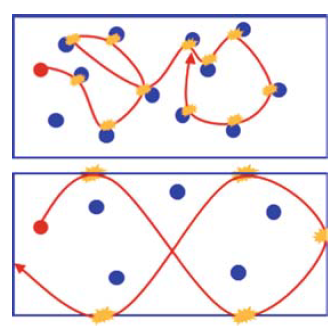
\includegraphics[width=0.4\textwidth]{1.png}
\caption[ballistic]{Path of a heat carrying particle (\textit{red} blob) in the diffusive regime (\textit{top}), where the carrier
density is high, and in the ballistic regime (\textit{bottom}), where the carrier density is low. The prevailing
mechanism in the diffusive case is interparticle interaction. In the ballistic case, it is particle–
surface interactions that dominate\cite{mingolbook}}
\label{fig:mingo}
\end{figure}{}

In a first approximation, reflection and transmission are assumed to be a linear
combination of the two extremes, specular and diffuse. The fraction of the incident
energy that is reflected specularly defines a coefficient called the specularity. But
while the particle on its straight line path is indeed treated as a particle, it is its
wavelike behaviour that governs its reflection or transmission. The specularity coefficient
will thus depend on the wavelength and polarisation of the particle, the
roughness of the surface, and the angle of incidence. It is therefore impossible to
account exhaustively for the full complexity of the physical mechanisms that contribute
to this coefficient, and it is generally treated as a floating parameter when
computations are carried out.\\
\indent This first rarefaction effect is often computed using the Boltzmann equation, which is exactly what we conduct with MC methods in Chapter 2.
\subsection{Confinement}
The word ‘particle’ is used to cover the more detailed reality of a localised wave
packet. This wave packet is made up of several waves in different resonant or normal
modes. It is the mode, the manner of vibration, that contains the energy of the
system. It is assumed to be a travelling wave, since the system is a bulk system and
much bigger than the lattice constant, i.e., the interatomic distance. The amplitudes
$u_n$ of these waves can be modelled by plane monochromatic waves, that is, complex
exponentials whose arguments contain the wave vectors $k$ and a time dependence associated with the frequency $\omega$:
\begin{equation*}
u_n=ue^{i(kx-\omega t)}
\end{equation*}
When modelling such modes, the boundary conditions are called Born–Von Karman
conditions: the wave arriving at one end will come back in by the other. It thus
propagates indefinitely in the same direction as long as it does not interact, and it
moves at a speed imposed by the speed of the given mode.\\
\indent Imagine now that the wave amplitude is annihilated at one end. This is what happens,
for example, at the bridge of a guitar or when an acoustic wave in a crystal
arrives at a free surface. The wave incident at this stopping point will be reflected
with reversal of its phase. The incident and reflected waves
can still be modelled by monochromatic plane waves, that is, complex exponentials
whose arguments contain wave vectors k with opposite signs, since the waves propagate
in opposite directions. Their superposition is thus modelled as a sum of two
exponentials, equal to the product of a cosine function whose argument depends on
the wave vector and a complex exponential defining the temporal phase:
\begin{equation*}
u_n ~ e^{i(kx-\omega t)}+e^{i(-kx-\omega t)}= cos(kx)e^{-i \omega t}
\end{equation*}
The zeros of the cosine function do not depend on time and define the nodes of a
stationary wave. The vanishing of the amplitude at the boundary $x=L$ requires $kL=\pi /2+n2\pi$, where $n$ is an integer\cite{mingo2005carbon}. The wavelengths are thus $L/(n+1/4)$, defining
the normal modes of the cavity formed by the structure. If the width $L$ varies, then
the wavelengths will also vary. New eigenmodes specific to the nanostructure thus
form.\\
\indent This transformation of the travelling normalmodes into stationary normalmodes
is the second non-Fourier effect, referred to as confinement. By definition, these
stationary waves have zero propagation speed. As the heat flux is proportional to
the speed, the contribution of such stationary modes to heat transfer also vanishes The dispersion curves giving the frequency as a function of the wave vector are
therefore flat, because their slope is given by the mode speed, as shown in Fig(\ref{fig:mingopic}).
\begin{figure}[htbp!] 
\centering    
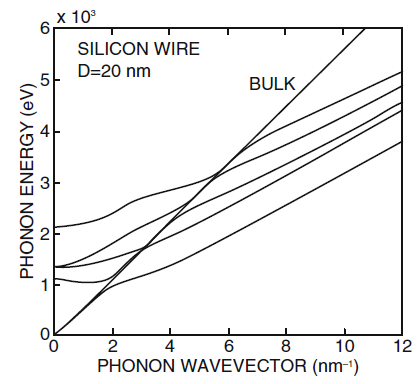
\includegraphics[width=0.4\textwidth]{2.png}
\caption[confinement]{Dispersion curves for the phonons in a silicon nanowire of diameter 20 nm (\textit{continuous
lines}). Small slopes and low group velocities correspond to small phonon wave vectors or long
wavelengths as a result of confinement. Each branch is related to the projection of an oblique mode
onto the wire axis. The bulk dispersion curve is shown by the \textit{dashed line}.\cite{mingolbook}}
\label{fig:mingopic}
\end{figure}{}
\subsection{Density of States and Dimensionality}
As can be shown from Fig(\ref{fig:mingopic}), confinement modifies the distribution of the modes
as a function of frequency. The number of modes in a given frequency interval$[\omega, \omega + d \omega]$ or wave vector interval $[\textbf{k},\textbf{k}+d^3 \textbf{k}]$ is called the density of states $D(\omega)$ or $D(k)$, respectively.\\
\indent The directions of the vibrations in a crystal cover the whole space, and so do the
directions of the wave vectors. The density of states in the bulk is thus proportional
to a volume element, let us say an element in the form of a spherical shell, i.e., $D(k) \propto k^2 dk$. If now the vibrations only build up in two dimensions, as in a graphene
film, the density of states is proportional to a surface element, i.e., $D(k) \propto k^2 dk$.Finally, in the case of a nanowire, where the vibrations can only propagate in one
direction, the density of states is proportional to a length element, i.e., $D(k) \propto k dk$.\\
\indent Since the thermal conductivity is proportional to the heat capacity, and
hence to the density of states, the dimensionality of the structure has a significant
impact on heat transfer. 

%\section{Interface}
%After discussing all the three non-Fourier effects and getting a overall view of the nanoscale heat transfer, we will turn to focusing on the topic of interface, which becomes increasingly important on small length scales.  

\section{Solid-State Lighting: Focusing III-V semiconductors}

The interactive progress in semiconductor science and technology has transformed and continues to transform both our scientific understanding of the universe and the technologies with which we live our daily lives\cite{LEDblue}. A testament to this are the seven Physics Nobel Prizes listed in Fig(\ref{fig:LEDnobel}) that have been awarded in the broad area of semiconductors.
\begin{figure}[htbp!] 
\centering    
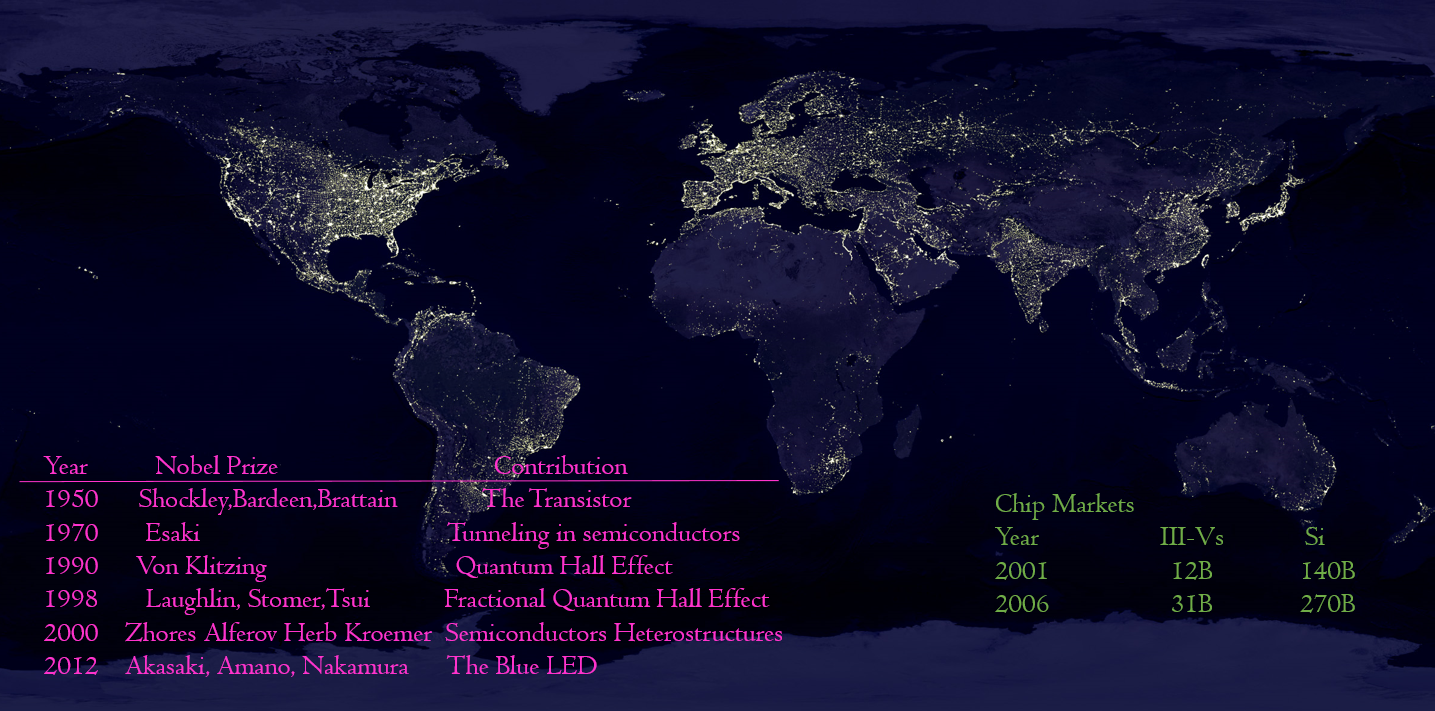
\includegraphics[width=0.8\textwidth]{NASA.png}
\caption[semiconductorsNobel]{Timeline of Physics Nobel Prizes in semiconductor science and technology}
\label{fig:LEDnobel}
\end{figure}{}
Some of the Prizes were for technology
breakthroughs – as with research
surrounding Si planar processing
and the integrated circuit.
Some of the Prizes were for science
breakthroughs – as with research
surrounding the integer and
fractional quantum Hall effects. And
some were for nearly simultaneous
science and technology breakthroughs
– as with the transistor.\\
\indent The most recent 2014 Physics Nobel Prize, for the blue light-emiting diode(LED), is clearly for a technology breakthrough. Indeed, this makes it possible to gain relaible and clean light and thus bring about a Solid-State Lighting revolution.Because artificial lighting is so critical to humanity and consumes so
much energy (approximately 6.5\% of
the world’s primary energy and 16\%
of the world’s total generated electrical
energy \cite{LEDworld}), the energy savings
potential of SSL is huge.\\
\indent During all the types of semi-conductors, when we talk about Optoelectronics, the III-Vs can be very unique.
The uniqueness and practical importance of the
compound III-V semiconductors stems from their
balancing of these competing trends. They are
polar enough to be direct-bandgap semiconductors,
with the accompanying strong interactions with
photons useful for optoelectronics and the low
electron masses useful for high-speed electronics.
But they are not so polar that they cannot be p-type
doped or that they suffer from too-high defect
densities.Thus, III-Vs semi-conductors gain vital importance in the area of LED or other Optoelectronics.\\
\indent Also, as we have mentioned in the Intro, the rapid development of Optoelectronics especially the nano III-V structures demands a deep understanding of the phonon transport and then tuning the heat condcution, which is the basic background of our whole research. So in this part, we will then focus on the most important part of the nano structures-interface and will continue this topic in late chapters.
% \section{Thermal Conductance of Inteface}
% %\subsubsection{Vibrational thermal energy transport at interfaces}
% Interfaces play a key role in the thermal behavior of nanostructures. At small scales, interfaces have the potential to become the dominant resistance to heat conduction, which impedes the progress towards achieving improved performance in nano-electronics\cite{pop2010energy}, nano-optoelectronics\cite{tien1994challenges}, or energy conversion devices such as multi-junction solar cells\cite{min2009thermal,katz2006effects}.
% A thermal boundary resistance is found for the heat flow
% between two materials in contact along a planar interface.
% The heat flow is perpendicular to the planar interface
% \begin{equation}
% J_Q=G \Delta T
% \end{equation}
% where $\Delta T$ is the small temperature difference between the two sides of the interface, and $G$ is the boundary conductance; $G$ has the units of power per aera per degree.\\
% A common interface in thermal transport is bettween two insulators. Then, the heat is carried only by phonons. The accoustic model(AMM)\cite{little1959transport} and diffusive mismatch model(DMM)\cite{swartz1989thermal} have traditionally provided a basis for understanding interfacial thermal resistance. These models provide prescriptions for calculating the transmission coefficient of a phonon with which the interfacial conductance can be obtained by appropriate summations over all phonons\cite{young1989lattice,swartz1989thermal}.\\
% As a continuum model, the AMM assumes that phonons
% undergo specular reflection or transmission at the interface.
% This model is valid in the long-wavelength limit, where
% due to their small details compared to the incident phonon
% wavelength, interfaces are seen as sharp. The DMM, on
% the other hand, assumes not only purely diffuse scattering
% at the interface, but also an equivalence between phonon
% reflectance from one side to the transmittance from the other.
% This model, as opposed to AMM, is valid for very rough or
% dirty interfaces and short-wavelength phonons. Neither AMM
% nor DMM consistently predict interface thermal boundary
% resistance.\\
% For the late discussion it should be pointed out here that while both AMM and DMM provide values
% for transmission coefficients, they calculate them purely
% based on the bulk properties of the two solids forming the
% interface; thus they do not account explicitly for the strength of the interfacial bonding. 

\section{My Oric Study}
After giving the introduction above, we can conclude that nanoscale thermal transport plays an important role in the functionality and the reliability of nano-enabled systems. However, we must realize that the understanding of nanoscale thermal transpoat is still in its infancy.\\
\indent The key to the difference in thermal transport at nanoscale from that at macroscale is the scattering of energy carriers at interfaces. And we have also introduced the two well-known model DMM and AMM which have been widely-used to describe the phonon properties in interfaces, however, in many realistic systems, just the macroscopic properties, which the two models only contain, such as interfacial thermal resistance and the reduced thermal conductvity of nanostructures, could not caputure all the underlying physics\cite{yang2004thermal,yang2005thermal}.For example, a large-scale nano-bulk system with multiple interfaces such as intergrated circuits(\textbf{ICs})\cite{IC} and nanocomposites\cite{yang2005thermal} will call for a better set of variables and simulation tools to describe such a system. Empirical approaches are the Boltzmann transport equation-based determinstic andstochastic approches, which could potentially link the length scales from a few nanometers to the macroscale\cite{LD2}. And we will also conduct a MC simulation based on phonon BTE mainly to recover the picture of the nano-scale heat conduction and in this work we also consider the effect of the internal heat source which can be a good model for many actual nano-thermal devices, for example, chips.\\
\indent Although such simulations gain great success in several topics, tools like MC simulation require input parameters that must be obtained at even smaller length scales, such as the phonon relaxation time, phonon dispersion, and phonon transmission coefficent at interfaces(These can be seen from Chapter 2 and Appendix A ). Most of these input parameters(material properties at atmistic scale) are energy or wavevector(actually these two are same). More importantly, various factors, such as material differences, atomic reconstruction at the interfacial region, dislocations, defects, strain fields, and the size of the structures, could affect these parameters, including phonon transmission across interfaces of dissimilar materials\cite{li2012size}.\\
\indent Modeling of phonon transmission across material interfaces has been challenging. The acoustic mismatch model(AMM) and diffuse mismatch model(DMM) are often used for the calculation of phonon transmission as input parameters for Boltzmann equation solvers\cite{DMM}.
The AMM considers long-wavelength phonons and uses the acoustic impedances of the two adjacent materials for the calculation of phonon transmission. The model is strictly valid only at low temperatures. Phonon scattering at interfaces is assumed to be completely diffusive in the DMM\cite{DMM},which relates the
phonon transmission to the mismatch of the phonon density
of states (DOS) of two materials. The DMM better predicts
phonon transmission at high temperature or across rough
interfaces. Although the AMM and DMM have been used
exclusively for BTE solutions and for explaining experimental
data, neither the AMM nor the DMM can accurately capture
the underlying physics of phonon dynamics and transport
across material interfaces.\\
\indent Significant progress has been made recently in studying	phonon transmission based on atomistic simulations. The
phonon wavepacket method\cite{schelling2002phonon} was developed to study
phonon transmission based on molecular dynamics (MD)
simulations. In this method, a phonon wavepacket is
initiated in one material and propagates across the interface.
Wavefunctions with specified wavevector and frequency are
used to assign the initial displacement and velocity of the
atoms. The transmission coefficient is calculated by the
ratio of the total energies (both potential and kinetic) of
the atoms on the two sides of an interface.However, usually the
simulation domain is very large in the direction perpendicular
to the interface\cite{schelling2002phonon,sun2010molecular}.For example, a size of 543 nm
is used in work\cite{schelling2002phonon}, and only one phonon transmission data
point corresponding to a specific phonon wavevector can be
obtained in one run of MD simulation.It is rather costly for obtaining the phonon transmission for all phonon modes.\\
\indent Linear lattice dynamics\cite{stoner1992measurements,zhao2005lattice} was proposed to
calculate phonon transmission using the lattice dynamical
equation derived for the atoms at the interface. Under the
harmonic approximation, the frequency of the transmitted
and reflected phonons does not change. With this boundary
condition, the wavefunctions of the reflected and transmitted
phonons can be solved and then the phonon transmission
is calculated based on the energies of the reflected and
transmitted phonon waves across the interface.\\
\indent Instead of solving for phonon waves in the linear
lattice dynamics method, the atomistic Green’s function
(AGF) approach solves for the response of the system
under small perturbations. In the AGF approach, a lattice
system is divided into decoupled sub-systems. The Green’s
functions of the decoupled sub-systems are obtained first
and the Green’s function of the coupled system is then
calculated by linking the Green’s functions of the decoupled
sub-systems. In this way, if there is any change in one of
the decoupled sub-systems, only the Green’s function of
this decoupled sub-system needs to be recalculated and the
new Green’s function of the whole system can be relatively
easily calculated by replacing the Green’s function of this
sub-system, which is more computationally efficient than
the linear lattice dynamics method. A number of interfacial
structures have been studied using the AGF approach,
including low-dimensional molecular chains, coated silicon
nanowires (NWs), amide-linked carbon nanotubes, latticematched
Si/Ge interfaces and rough interfaces of two
face-centered cubic (fcc) lattices\cite{ozpineci2001quantum,zhao2009phonon,dhar2006heat}.\\
\indent As we have mentioned above, it is far from enough to only consider bulk or macroscale properties to explain the interface mechanism, however, few studies have addressed this problem. So in our work, whose background is Optoelectronics, we set the final goal to further understand the deeper mechanism and physics in interface and this report focus on the phonon properties in III-V semi-conductors and also the heat transfer in these nano-structures. The paper is organized as follows.
In Chapter 2, the phonon MC method with the internal heat source is presented to mainly show the different temperature profile and the nano-heattransfer effects. In Chapter 3, we present the phonon transmission across the III-V semi-conductors interfaces. In Chapter 4, concludes the work and list the two undergoing work on that issue in our further study.


%!TEX root = ../thesis.tex
%*******************************************************************************
%****************************** Second Chapter *********************************
%*******************************************************************************

\chapter[MC Method]{A Monte Carlo simulation for phonon transport within silicon structures
at nanoscales with heat generation}

\graphicspath{{Chapter2/}}

%\section*{MC Work Abstract}
\setlength{\epigraphwidth}{0.6\textwidth}
\epigraph{“Anyone who wants to analyze the properties of matter in a real problem
might want to start by writing down the fundamental equations and then
try to solve them mathematically. Although there are people who try to
use such an approach, these people are the failures in this field. . . "}
{\textit{Richard Feynman, sugar coating it.}}


\textit{In nanostructures whose characteristic lengths are comparable to the phonon mean free path(MFP), the ballistic-diffusive heat conduction leads to the size effect\cite{hua0}, which means the relationship between the heat flux and the temperature becomes complicated.In this work, an effective Monte Carlo(MC) method on the basis of using a model of phonon scattering process is employed to simulate the ballistic-diffusive heat conduction in silicon nanofilms, which is based on the methods proposed by Hua's work to study the effective thermal conductivity of nanostructures with internal heat source in one dimension\cite{hua0,hua1}.To get a clear vision of the temperature distribution of the chip, I first calculated the phonon transport in a two-dimension silicon nanofilm with internal heat source. The simulation agrees with the the diffusive approximation(Kn<<1), and it clearly shows the size effect in two dimensions.}                
 
%%%%%%%%%%%%%%%%%%%%%%%%%%%%%%%%%%%%%%%%%%%%%%%%%%%%%

\section[Introduction]{A brief introduction}
As the rapid development of microelectronics, an in-depth understanding of nanoscale thermal transport is quite necessary\cite{Dames,hua2}. On one hand,the typical size of the electronic devices have been decreasing at a dramatical speed, just using the example of diode, which is the key component of chips. As is reported in October, 2016, $MoS_2$ transistors with 1-nanometer
gate lengths has been made out\cite{Desai}. On the other hand, the integration of single chip has been doubling per 18 months since the 1950s, causing the heat flux density arrives at as high as $10^5W/cm^2$, which makes it even harder for the cooling of the chips and electronics. Additionally, when the size of silicon decreases to micro even nano scale, the well-known law of heat transfer, namely Fourier's Law fails. The reliability of electronics, however, is sensitive to the temperature fluctuations. When the temperature reaches 70-80 $^\circ$C, the reliability will decrease 5\% if temperature becomes 1 $^\circ$C higher\cite{Flik}. Consequently, great efforts have been devoted to study the phonon transport phenomenon in micro/nano structures, especially the ballistic-diffusive heat conduction in silicon in recent years.\\
\indent Speaking of the heat transport in dielectric material, the heat transport is predominant by phonons which are quanta of crystal vibrational energy\cite{Statisticalmechanics,Ziman}.In bulk materials, phonons usually undergo several scatterings during the transport and the control law is the Fourier's law, $q=-k\nabla T$, where q denotes the heat flux , T denotes the temperature and k is the material constant of heat transfer. While in nanostructures, the characteristic lengths are compatible to the phonon mean free path(MFP), whose physical meaning is the mean distance a phonon can go before scattering occurs, causing some phonons will not undergo scattering before arriving at the boundary, which we call the ballistic transport. Actually, when the size reaches the nano scale, the effect of the boundary becomes quite important and cannot be omitted, and that is the reason why the governing rule and physical picture of nanostructures are so different from in bulk materials. In summary, the heat transport in nanostructures violates the classical rule, and we call the new process the ballistic-diffusive heat conduction.\\
The key point to solve the ballistic-diffusive conduction problem is to solve the famous equation proposed by Boltzmann\cite{Bolt}:
\begin{equation} 
\frac{\partial f}{\partial t} + v_g \nabla f = \frac{f_0 - f}{\tau} + \dot{S}_{\Omega} \label{con:Boltz}
\end{equation}
In which $v_g$ is the group velocity of phonon, f is the phonon distribution function, $f_0$ is the equilibrium distribution function(since phonons are boses, the Bose-Einstein distribution\cite{chandler}),$\tau$ is the relaxation time and $\dot{S}_{\Omega}$ the phonon source per solid angle\cite{hua3}, or more clearly, the internal heat source. What we should notice is that the effect of boundary is not directly included in this equation but its effect will be considered when we impose the boundary conditions when solving that equation.\\
\indent The temperature profile, which is an important point in this problem, is the focus of my work. Studies to gain the better picture of the temperature profile in silicon with internal heat source have been conducted both theoretically\cite{Lu,Amon} and experimentally\cite{Li,hsiao2013observation,Jo}. It has been found that in the ballistic-diffusive regime, if we still get an effective k(which is quite different from the k in bulk material, we just divide the heat flux by temperature gradient, namely, $k_{eff}=q/\nabla T$), significantly reduces as compared to the bulk material. One direct result is the on the condition of the same heat flux, the nano material will get a higher temperature rise compared to the temperature gradient predicted with the bulk material model, which is an urgent issue in electronic cooling.\\ \indent Although these both aspects have made great progress these years, the underling mechanism of the size effect is ambiguous and the general model with concrete physical base to predict the size effect and related other things is still lacking. So several simulation methods and techniques have been developed to help solve the problem.\\
\indent Three types of methods have been adopted to help simulate the phonon ballistic transport using Boltzmann transport equation(BTE): molecular dynamics(MD)\cite{MD},Lattice-Boltzmann method(LBM)\cite{LB} and Monte Carlo(MC)\cite{KL}. Compared with the MC method, MD method is limited in the size for its amount of calculation
and LBM is not suitable for simulation of complicated boundaries. MC method, which is a quite universal method in computational physics, has gained great success in solving many models in quantum and statistical mechanics\cite{Lan}. In our problem, we trace a great number of phonons(usually greater than $10^6$ and also depends on the size of the problem), derive the distribution function through statistics and then get the thermal properties of the material. In a nutshell, MC method actually give a discrete solution to the BTE and thus is more powerful when it comes to the effect of scattering and different boundary conditions.\\
%My highlight
\indent Our work aims at getting the temperature profile of the actual electronic chips, and based on that we can consider some methods to do the optimization. Considering most optimization of chips till now are actually conducted in macro scale, the attempt to do that work in nano scale can help better understand and finally solve the cooling problem.

%%%%%%%%%%%%%%%%%%%%%%%%%%%%%%%%%%%%%%%%%%%%%%%%%%%%%%%%

\section{Methods}
\subsection{Monte Carlo simulation details}
\subsubsection{The gray approximation}
For simplification, we choose the gray approximation in the MC simulation, which has been proved effective and acceptable in past work\cite{hua0,hua1}. The gray media approximation assumes that the phonon properties are frequency-independent, that's to say, the dispersion relationship of phonon is easiest and the $p$ just equals a constant. On operation, we can first get the dispersion relationship of phonon in silicon by quantum mechanics or doing experiments and then find out the frequency interval of which phonons carry the most of the energy to get the typical frequency we choose in MC simulation. Hence, we finally focus on the phonons traveling with one single velocity and we can study the scattering using one average MFP(These point is quite important for us to get the simplified BTE, namely Equation (\ref{con:Boltz})).\\
\indent It is well-accepted to choose the phonon MFP of bulk material, $l_a$, to do the MC simulation. $l_a$, can be calculated using the method of the kinetic theory.
\begin{equation} \label{eq2}
l_a=\frac{2 \lambda_{b}}{C_v v_g}
\end{equation}
where $\lambda_{b}$ is the thermal conductivity of bulk silicon, $C_V$ is the heat capacity whilst keeping the volume constant, $v_g$ is the average group velocity.
For silicon at room temperature, we list the main data in the following chart\cite{Super}.\\

\begin{table}[!hbp]
\centering
\begin{tabular}{|c|c|}
\hline $\lambda_{b}$  &150 W/(m k)\\
\hline $C_v$ & 1.63 $\times 10^6J/(m^3$ k) \\
\hline $v_g$&6400 m/s\\
\hline    
\end{tabular}\\
\caption{Silicon}
\end{table}

But if we explore the dispersion model of phonon in silicon more detailed, we will find the phonons in silicon can be divided into two types of phonons: acoustic phonons and optical phonons. If we only consider the acoustic phonons that carry most of the energy(that is acceptable in room temperature or we only need to consider the optical phonons at ultralow temperature), we get a new value of MFP, 260nm\cite{Super}. Actually, when we consider that new dispersion model, we need to change the corresponding $C_V$ and $v_g$,finally we choose the value at 43.7 nm\cite{hua1,hua2,hua3}.\\
\subsubsection{Relationship between energy and temperature}
We use the MC method to trace the phonons in the nanofilm and we can get the distribution, but we need to know the relationship between the distribution and the temperature to get the temperature profile.
Similar to the photon, the phonon intensity emitting from a black boundary has the form of what is famous as Stephen-Boltzmann rule\cite{HT}(The similarity also lies in the two quasi-particles both being Boses)
\begin{equation} \label{eq3}
E=\sigma T^4
\end{equation}
where$\sigma$ is a constant related to the material.
As for the internal unit, we can also derive the phonon intensity emitting imitating the theory of participating media radiation\cite{Thermal}, which can be written as
\begin{equation} \label{eq4}
dQ_{em}=4\epsilon \sigma T^4 dT
\end{equation}
where $\epsilon$ is the phonon emissivity($\epsilon$=$l^{-1}_a$). Because we consider the equilibrium state, the phonons received from the boundaries and all the other unit control volumes are equal to those emitting from the internal heat source. Thus, if we accept the local thermal equilibrium assumption, we can then get the local temperature.\\
\subsubsection{The sampling method}
As we all know, although the MC method is powerful and seems easy to employ, the sampling of particles is of critical importance in the simulation not only because the sampling method differs greatly as the system changes but also because this is important for the feasibility of MC simulation(We can expect a dramatic decrease in the calculation if a suitable sampling method is adopted). So then we will discuss which sampling method we will apply in this problem.\\
\indent We can define the intensity of each phonon bundle emitting as
\begin{equation} \label{eq5}
W=\frac{E}{N_p}
\end{equation}
It should be pointed out that $N_p$, which is the number of the phonon bundles we trace, must be large enough to preserve the simulation accuracy\cite{New}(According to the MC method, we can minimize the fluctuation if the number of particles is large enough).\\
\indent Usually, we discuss the phonon transport in a ball coordinate, so in this coordinate, the traveling direction vector of the phonon bundle is given by
\begin{equation}  \label{eq6}
\textbf{S}=[\sin{\theta}\cos{\phi},\sin{\theta}\sin{\phi},\cos{\phi}]
\end{equation} \\
How to sample the bundles of phonons to set the information of $\psi$ and $\theta$ is the key issue in this step. Since the study on radiation whose energy carries are photons has been detailedly conducted, as we did before, we can get the relationships between the angles and independent random numbers according to Ref\cite{}.
\begin{enumerate}
\item When the phonon bundle emits from the boundary, $\sin{\theta}=(R_{\theta b})^{1/2}$,~$\phi=2 \pi (R_{\phi b})^{1/2}$
\item When the phonon bundle travels in the media, $\cos{\theta}=1-2R_{\theta m}$,~$\phi=2 \pi (R_{\phi m})^{1/2}$
\end{enumerate}
We need notice that $R_{\theta b}$~$R_{\phi b}$~$R_{\theta m}$~$R_{\phi m}$ are independent random numbers ranging from 0 to 1 and can be generated by computer programs.\\
\indent Because we mainly consider the stable status which is also the normal state in actual chips, we can divide the scattering of phonons into only two parts, one is phonon-interface scattering and intrinsic scattering. We need to note that the boundary scattering is actually quite complicated and I will discuss it in later paragraphs. Now we just need to know, we have two types of boundaries in this simulation, one the black-body where the phonons will be completely absorbed, the other adiabatic where we assume phonon scattering can be equivalent to a diffuse reflection
process which means phonon will be absorbed and then randomly remitted.Furthermore, speaking of the intrinsic scattering, such as phonon-impurities, phonon-phonon and phonon-electron scattering, can be treated wholly in the relaxation time approximation. According to Hua's work\cite{Acta}, the average travel distance of phonon bundle can be calculated as
\begin{equation} \label{eq 7}
\Delta l=-L Kn \ln{ (1-R_{s})}
\end{equation}
Based on the definition of kn number (kn=$\frac{MFP}{l_{typica}}$), we can know if the scattering the phonon bundle undergo is the same as in the bulk material, l=MFP. In nano structures, the scattering is quite stronger than in bulk material so the actual traveling distance will be quite different.\\
\indent The last item  is the tracing algorithm which is shown in Fig \ref{fig:1} .
\begin{figure}[!hbt]
  \centering
  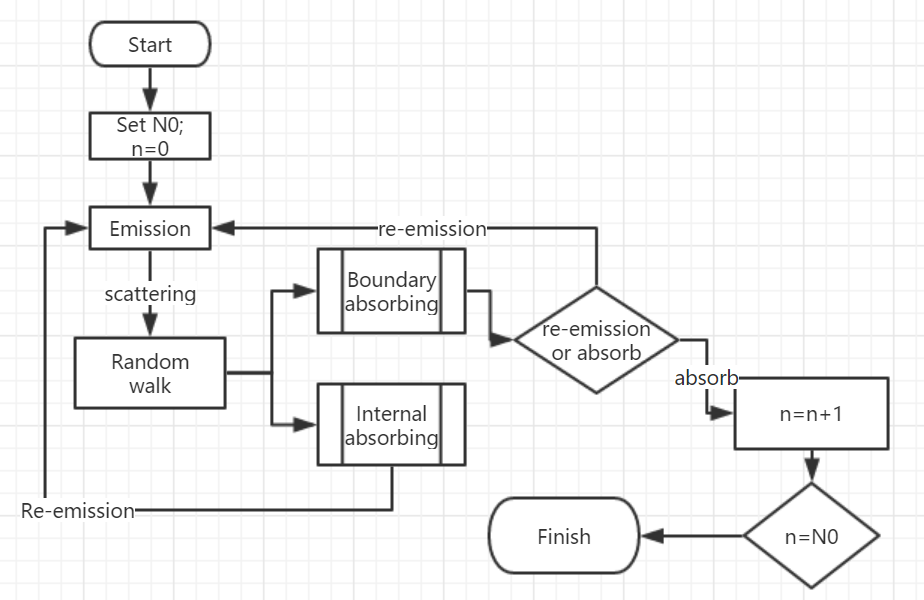
\includegraphics[width=3in]{1.png}
  \caption{Block diagram of the tracing algorithm}
  \label{fig:1}  
\end{figure}


\subsection{Monte Carlo simulation steps}
\subsubsection{Problem formation}
The Two dimensional thermal transport in silicon films with internal heating can be characterized by the two dimensional BTE, $\partial f / \partial t + V_{gx}\partial f / \partial x + V_{gy}\partial f / \partial y = (f_0 - f)/ \tau + \dot{S}_{\Omega}$. 


\begin{figure}[!hbt]
  \centering
  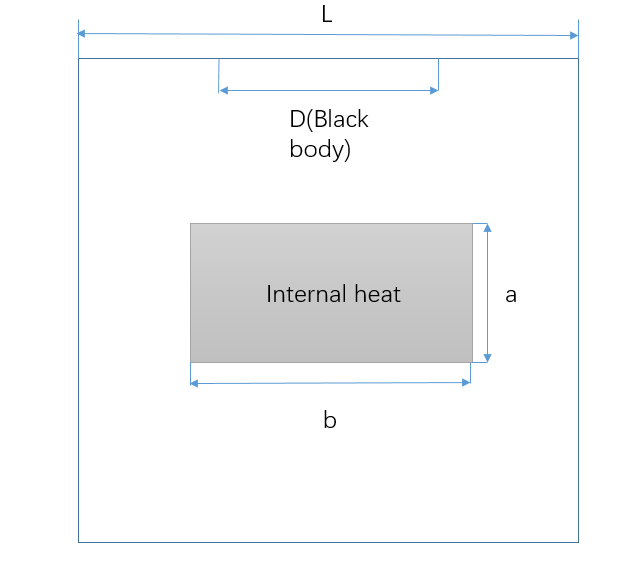
\includegraphics[width=2.5in]{5.png}
  \caption{Two dimensional thermal transport in silicon films with internal heating}
  \label{fig:2}  
\end{figure}

The schematic of simulating object is illustrated in Fig \ref{fig:2}.The upper boundary with the length of D is considered as phonon blackbody, that is to say, phonon are completely absorbed there, which means heat will only conduct to outer space there, while all the other boundaries are adiabatic and the phonon-boundary scattering at them is assumed to be completely diffusive.The internal heat source is implemented by setting the phonon source inside the nanofilms, which is clearly shown in the Fig, and phonons with definite energy will originate within the zone.Then, all the phonon bundles will be traced until they exit through the black-body boundary. \\
\indent The temperature profile then can be obtained from the phonon distribution calculated by our MC simulation\cite{hua1}. More importantly, we should note that since our system is comparable with the phonon MFP, the local thermodynamic equilibrium cannot be established, and the temperature is more a parameter than its conventional meaning of representing a thermal equilibrium state.\\
\indent One famous theory proposed that in that case, the temperature calculated is actually a representation of the average energy of all phonons around a local point\cite{Super}. And we will adopt that explanation and will give our temperature profile according to that.
\subsubsection{Monte Carlo simulation}
The MC technique simulates phonon transport process by random number samplings, equivalent to directly solving the phonon BTE. The phonon tracing algorithm is as follows:
\begin{enumerate}
\item Draw the initial properties(by randomly choose a point in heat source zone) ,for example, $r_0$ of phonon bundle.
\item Calculate the traveling length using the Eq(7), and renew the position of the phonon, $r_{new}=r_0+\Delta r$.
\item If a phonon collides with a boundary, if it is the black-body boundary, set n=n+1(n denotes the number of phonons which emit),or at the adiabatic boundary then
 set the position value at the boundary and let the phonon re-emit from the boundary.
 \item If a phonon does not collide with the boundaries, the phonons just re-emit at $r_{new}$, and we set $r_0=r_{new}$.
 \item Record the frequency phonons get absorbed at each control body(each grid) and when n equals $N_p$($N_p$ is the number of the phonon bundles we trace in simulation), the whole process is finished.
\end{enumerate}
Just one thing should be noticed, although we choose a large number of phonon bundles, we trace only one at a time. When a phonon exits at the black-body boundary, we emit another and repeat till all the phonon bundles has been traced and recorded.

\section{Results}

%\section{Results and Discussions}
\subsection{Results and discussion}

\begin{figure}
\begin{minipage}[t]{0.33\linewidth}
\centering
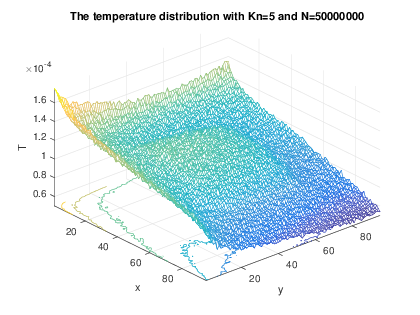
\includegraphics[width=2.2in]{2.png}
\caption{Kn=0.05}
\label{fig:3}
\end{minipage}%
\begin{minipage}[t]{0.33\linewidth}
\centering
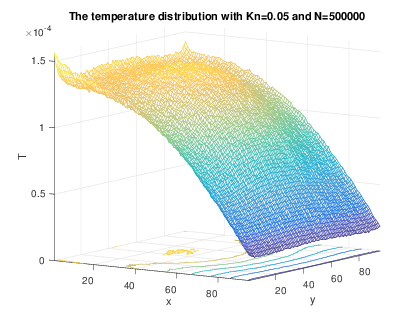
\includegraphics[width=2.2in]{3.png}
\caption{Kn=0.5}
\label{fig:4}
\end{minipage}
\begin{minipage}[t]{0.33\linewidth}
\centering
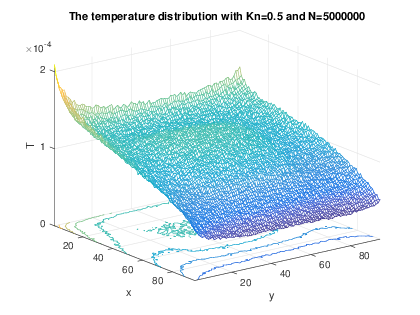
\includegraphics[width=2.2in]{4.png}
\caption{Kn=5}
\label{fig:5}
\end{minipage}%
\end{figure}

\begin{figure}
\begin{minipage}[t]{0.5\linewidth}
\centering
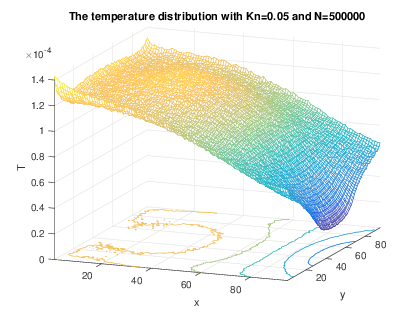
\includegraphics[width=2.2in]{6.png}
\caption{Kn=0.05}
\label{fig:6}
\end{minipage}%
\begin{minipage}[t]{0.5\linewidth}
\centering
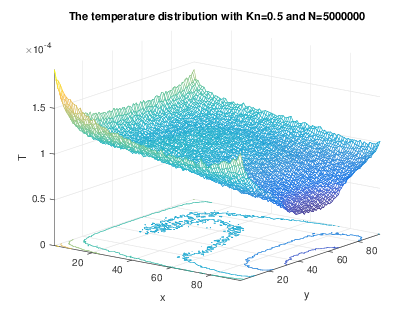
\includegraphics[width=2.2in]{7.png}
\caption{Kn=0.5}
\label{fig:7}
\end{minipage}
\end{figure}

The dimensionless temperature profiles in Si nanofilms are shown in Fig \ref{fig:3},Fig \ref{fig:4},Fig \ref{fig:5}.As Kn = 0, the phonon transport is purely diffusive and the corresponding temperature profile can be calculated by the classical   law. With the increase of the Knudsen number, phonon ballistic transport becomes stronger.
The temperature jumps occur at the boundaries and the temperature
gradient becomes smaller.And we can find there exits a temperature jump between at the boundaries and increase with the Knudsen number.\\
\indent We can conclude that when the kn gets closer to $\infty$, there will be no temperature gradient in the nanofilm and will result a highest temperature jump on the boundaries.\\
\indent And we can know when the kn Number becomes bigger, the scattering decreases and thus it gets harder to reach the equilibrium, so we increase the sampling number from 50,0000 to 5000,0000 as the kn ranges from 0.05 to 5.\\
\indent One thing should be added is the perturbation at the boundary is mainly caused by the truncation error of the computer and we just give up some units to correct and that won't affect the whole temperature profile.




\subsubsection*{Boundary condition changes}
If we narrow the width that the phonons can pass,which are shown in Fig \ref{fig:6} and Fig \ref{fig:7} namely the black-body boundary, we can find the temperature profile will change and the temperature around the exit will be lower. That calculation means this method can be applied to more complex boundary conditions.\\

\subsection{Conclusion}
\begin{itemize}
\item Based on Hua's work on one-dimension study on conductivity which is focuses on the mechanism in the ballistic-diffusive transport, we develop this method to two-dimension and in the future to real devices by considering more complicated boundary conditions and influence.
\item The MC technique can help solve the BTE and gives a valid temperature profile in different Knudsen numbers which is the same with different MFPs in reality. And this will help us understand the heat conduction in nano-films and then develop the optimization.
\end{itemize}

\subsubsection*{Frequency-dependent MC Simulation}
Because we adopt the Gray-body approximation in our MC simulation, we don't consider the phonon frequency effect. However, it is found that, in the room temperature and the region we mainly care about, this a good for calculating the temperature profile. So in next chapter, we will focus a more crucial and interesting , also not fully covered aspect, the phonon properties in interfaces, which also plays a significant role in our goal of tuning the thermal conduction in nano devices.But we still 
summarize the main points of the frequency-dependent MC simulation in Appendix2.





\clearpage

% \footnote{My footnote goes blah blah blah! \dots}



\chapter{Interface Phonon Properties}

% \ifpdf
%     \graphicspath{{Chapter2/Figs/Raster/}{Chapter2/Figs/PDF/}{Chapter2/Figs/}}
% \else
%     \graphicspath{{Chapter2/Figs/Vector/}{Chapter2/Figs/}}
% \fi

\graphicspath{{Chapter3/}}
\setlength{\epigraphwidth}{0.6\textwidth}
\epigraph{“There are no real one-particle systems in nature, not even few-particle
systems. The existence of virtual pairs and of pair fluctuations shows that
the days of fixed particle numbers are over.”}
{\textit{Viki Weisskopf(American theoretical physicist)}}



\section[Introduction: Why we focus on interface]{Why we focus on interface}
\subsection{Research update: Heat conduction in nanostructured materials}  % also can get a short title like the \section
After we study the quasi-ballistic phonon transport in nano-films with MC method and get an overview of the temperature profiles in different 
knudsen Numbers, we have clearly observed the size effect caused by internal phonon scattering. And what should be pointed out is that in this former work we did not consider the effect of phonon boundary scattering in interfaces, but when it comes to actual device, multi-structured silicon devices have complex interfaces and experiments have demonstrated that in this regime, the surface or interface scattering becomes predominant compared to the internal scattering\cite{ChenRenkun,Hochbaum1}.\\
\indent Just as we have mentioned before, with the formidable and accelerated integration of transistor devices started in the sixties - about 9 billions CPUs are in function today - and the mid-heighties apparition of nanosciences, which finally benefited mostly to the materials
community, the question of the thermal management of small systems and of the micro-to-nanoscale thermal design of
materials led to the necessity of revisiting heat transfer principles\cite{Volz1}.
\\
\indent So we will turn to managment of multi-structured systems and focus on the phonon properties in interfaces. Althogh we employ the similarity of phonons and photons in our design of MC simulation algorithm, when it comes to the interface, phonons are more difficult to apprehend as they are non-local quasi-particles like photons\cite{zimanphonons}. Phonons
are strongly interacting together through inelastic or anharmonic three- or four-body interactions and there typical wavelength at room temperature remains lower than 10nm\cite{ChenRenkun} (whereas photon Wien’s wavelength is of ten microns). And in our focused regime, thermal wavelengths comparable to the system size lead to confinement, which in turn yields to a reduced phonon transport due to group velocity decrease but also to relaxation time modification\cite{kazan}.
\subsection{Status and Challenges:Multiscale phonon transport calculations}
In contrast to photonics, plasmonics or acoustics where a single mode can be excited and analyzed, the main difficulty in phonon heat conduction consists in the treatment of a broad band Planck’s spectrum reaching tens of TeraHertz where modes are thermally excited in all directions in the form of decorrelated wave packets strongly interacting together through complex selection rules. This challenging situation makes of heat conduction a very rich science involving solid-state, statistical, quantum and transport physics\cite{Volz1}.\\
\indent While the impact of surface and interface scattering has been shown\cite{VolzSeba}, the detailed descriptions of the phonon wave mechanisms occurring at the boundary remain to be established. Confinement effect, which was predicted\cite{Baltes,Montroll} before, has received strong proofs in nanowires, nanofilms\cite{kazan} and especially in superlattices\cite{Luckyanova,Ravichandran}.\\
\indent One important breakthrough to model  realistic phonon properties such as relaxation times is based on the DFT(density functional theory) approaches\cite{Ward}.
Compared with the MD method\cite{Ladd,Volz2} which has been widely used before and depends on the validity of the interatomic pseudopotential,the DFT method represents quantum populations and is discarding the contribution of free electrons.
However, the estimations remain limited to periodic or few atoms systems and also adopt many approximations such as single mean relaxation time and local near-to-equilibrium approximations. And this is why we choose to use classical potential to perform our calculations in later work, because doing calculations based on DFT is rather time-consuming, especially for lager systems. And also we will give a short introduction on Quantitative calculation from first principles based on density functional theory to compare with our AGF method based on the classical potential in Appendix2.


%\section*{Enumeration}
\section[Methodology: The Atomistic Green,s Function Method]{AGF: The Methodology}
\subsection{Introduction}
A growing interest exists in mesoscopic phonon transport, in which device dimensions becomes comparable to the typical wavelength of a phonon, and the wave nature of phonons becomes prominent. And as we have discussed above, phonon transport is often restricted by the heterogeneous boundaries and interfaces embedded in devices.In this quasi-ballistic transport regime, the atomistic Green’s function (AGF) method is efficient at handling interface and boundary scattering\cite{ATF}. The atomistic Green’s function approach combines atomic-scale fidelity with asymptotic treatment of large-scale (bulk) features, such that the method is particularly well suited to address an emerging class of multiscale transport problems\cite{ReviewATF}.\\
\indent Compared to other methods such as molecular dynamics (MD)\cite{MD1,MD2} and the phonon Boltzmann transport equation (BTE)\cite{BTE1,BTE2}, the atomistic Green’s function method is strictly valid at low temperatures. It accounts for boundary and interface scattering efficiently and offers great flexibility in handling complicated geometries\cite{ATF}.\\
\indent To set up a correct configuration we should notice that in a typical device-contact setup, contacts (or thermal reservoirs) play significant roles. Phonon distributions in contacts can significantly change the phonon transport characteristics of the device\cite{Angelesc}. That can be strictly met in AGF method because the AGF method uses self-energy matrices to represent the effect of bulk contacts on the device, thus simplifying the complexities of multiscale transport.\\
\indent One last thing before we turn to the details of the AGF method is that we need to know the two primary theories that have been employed to explain the mechanism of the thermal boundary resistance.One is the acoustic mismatch model (AMM)\cite{AMM}, and the other is the diffuse mismatch model (DMM)\cite{DMM}. Both models neglect atomic details of actual interfaces, and thus offer limited accuracy in nanoscale interface resistance predictions\cite{Stevens}. The AGF method can predict thermal boundary resistance between heterogeneous materials with full consideration of the interfacial atomic structures. And we will return to this topic in 3.4 and 3.5 when we consider and study detailedly on the ITC(interfacial thermal conductance)\\
\indent In the following part, a detailed mathematical
derivation of the phonon transmission function is provided in terms of Green’s functions and, using the transmission function, the heat flux integral is written in Landauer form. Within this theoretical framework, the required inputs to calculate heat flux are equilibrium atomic locations and an appropriate interatomic potential.

\subsection{AGF:Mathematical Formation}
\subsubsection*{General Description}
 First let us take a look at the common atomic structure of interest, which can be generalized as a device between two contacts, as shown in Fig\ref{fig:contact}.As is shown in the fig, Contact1(separated into two atom groups LCB and LC) and Contact2(separated into two atom groups RCB and RC) are two semi-infinite thermal reservoirs at constant temperature $T_1$ and $T_2$, respectively.And the Device includes three atom groups LD,D and RD, what is important is its geometry is arbitrary, which means it can be an atomic chain or a nanowire even a nanofim.\\
\indent The other thing about the setup is the connections.The types of connections between the device and contacts are arbitrary(point contact, limited contact or planar contact). And the difference between LCB and LC is atom group LC includes atoms that bond with Device atoms while LCB doesn't.That will bring out the difference of the dynamical properties of these two groups, LC and LCB in general heterogeneous system. And the bonds connection is the same at the right end. 


\begin{figure}[htbp!] 
\centering    
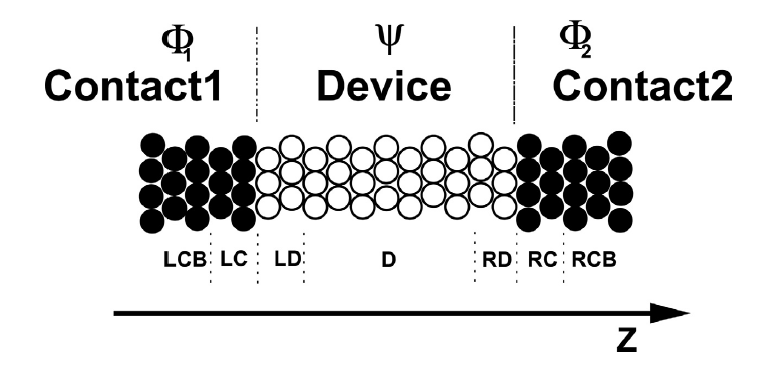
\includegraphics[width=0.6\textwidth]{contact}
\caption[contact]{Schematic diagram for a general contact-device-contact setup\cite{ATF}}
\label{fig:contact}
\end{figure}

\subsubsection*{Harmonic Matrix}
The AGF method\footnote{We mainly list the important formulas and omit the mathematical derivation} is founded on a harmonic matrix of the system of interest. Because prior work has shown that anharmonic scattering can generally be neglected at room temperature when the characteristic length of the device is less than 20 nm and we are focusing on atomistic structure of interface which usually consists of tens to hundreds of atoms, a harmonic matrix can be used to represent interactions among different degrees of freedom.The definition of the harmonic matrix in math is as follows\footnote{We use no Einstein summation rule in this article}
\begin{equation}
\textbf{H}={H_{pq}}=\frac{1}{\sqrt{M_p M_q}}\left\{\begin{array}{ll}
-\frac{\partial^2 U}{\partial U_p \partial U_q}&  \text{if p $\neq$ q},\\
-\sum_{m \neq q} -\frac{\partial^2 U}{\partial U_p \partial U_m} & \text{if p = q}.
\end{array}\right. \label{con:harmonic}
\end{equation}\\
In which $u_p$ and $u_q$ refer to any two atomic virational degrees of freedom (displacements,
momentums),respectively.U represents the total interatomic potential. What should be noticed, $M_p$ and $M_q$ are atomic masses associated with degrees of freedom $u_p$ and $u_q$. \\
Therefore, according to Solid Physics\cite{Ashcroft},the dynamic equation for the system can take this form
\begin{equation}
(\omega^2 \textbf{I}-\textbf{H})\tilde{u} = 0 \label{con:dynamic} 
\end{equation}\\
Where $\tilde{u}$ is a column vector consisting of vibrational degrees of freedom.And we note that though the assembled matrix $\textbf{H}$ can contain complex entries in complicated situations, its being Hermitian matrix guarantees that it has only real eigenvalues.

\subsubsection*{Green's Function Matrices}
Matrices $\tau_1$ and $\tau_2$ are used to represent interactions between two different atom groups. And the column vector $\psi$ and $\phi$, which can be seen in Fig\ref{fig:contact}, represent vibrational degrees of freedom in the device in contacts. We need to know that the number of degrees of freedom in the contact approaches infinity, so we use a sufficiently large number $n_c$ to approximate the number.$n_d$ and $n_c$ are degrees of freedom in the device and in interface regions(LC,LD,RC and RD).\\
We can derive the dynamic equations of the disconnected contacts based on Eq(\ref{con:dynamic})
\begin{equation}
[\omega^2 \textbf{I} - \textbf{$H_1$}] \phi_1^R=0
\end{equation}
\begin{equation}
[\omega^2 \textbf{I} - \textbf{$H_2$}] \phi_2^R=0
\end{equation}
where $\textbf{$H_1$}$ and $\textbf{$H_2$}$ are harmonic matrices of the two contacts.The superscript R means the disconnected state. We next use $\chi$ to denote the change to the original contact vector($\phi^R$), so after the contact and device establishes the connection, the actual contact vector becomes $\phi=\phi^R + \chi$.
Now the dynamic equation can be written together in matrix form:
\begin{equation}
\left[
\begin{matrix}
\omega^2 \textbf{I} - \textbf{$H_1$}&-\tau_1^{\dag}&0&\\
-\tau_1&\omega^2 \textbf{I} - \textbf{$H_d$}&-\tau_2&\\
0&-\tau_2^{\dag}&\omega^2 \textbf{I} - \textbf{$H_2$}&
\end{matrix}
\right]
\left(
\begin{matrix}
\phi_1^R + \chi_1\\
\psi\\
\phi_2^R + \chi_2
\end{matrix}
\right) = 0 \label{con:connect} 
\end{equation}\\
We can write the solution to Eq(\ref{con:connect}):
\begin{equation}
\chi_1=g_1\tau_1^{\dag}\psi
\end{equation}
\begin{equation}
\chi_2=g_2\tau_2^{\dag}\psi
\end{equation}
\begin{equation}
\psi=GS
\end{equation}
And the matrices$g_1$,$g_2$,G and S are defined next:
\begin{equation}
g_1=\lim_{\delta \to 0}[(\omega^2 + \delta i) \textbf{I} - \textbf{$H_1$}]^{-1} \quad (uncoupled\quad Green's\quad Function)
\label{con:g1} 
\end{equation}
\begin{equation}
g_2=\lim_{\delta \to 0}[(\omega^2 + \delta i) \textbf{I} - \textbf{$H_2$}]^{-1} \quad (uncoupled\quad Green's\quad Function)
\label{con:g2} 
\end{equation}
\begin{equation}
G=[\omega^2 \textbf{I} - \textbf{$H_d$}-\tau_1 g_1 \tau_1^{\dag}-\tau_2 g_2 \tau_2^{\dag}]
\end{equation}
\begin{equation}
S=\tau_1\phi_1^R+\tau_2\phi_2^R
\end{equation}
And we use $\sum_1$ and $\sum_2$ to denote $\tau_1 g_1 \tau_1^{\dag}$
and $\tau_2 g_2 \tau_2^{\dag}$,$S_1$ and $S_2$ to denote$\tau_1\phi_1^R$and$\tau_2\phi_2^R$.\\
Several matrices used later for convenience are defined as
\begin{equation}
A=i[G-G^{\dag}]=i[g_1-g_1^{\dag}]+i[g_2-g_2^{\dag}]=G\Gamma_1G^{\dag}+G\Gamma_2G^{\dag}
\end{equation}
\begin{equation}
\Gamma=\tau_1A_1\tau_1^{\dag}+\tau_2A_2\tau_2^{\dag}
\end{equation}
Where the first term and the second term of A can be denoted as $A_1$ and $A_2$, while the same with $\Gamma$,namely,$\Gamma_1$ and $\Gamma_2$.
In Eq(\ref{con:g1}) and Eq(\ref{con:g2}),i is the unitary imaginary number.And perturbation $\delta$ is very important and will be discussed next.
\subsubsection{Energy Flux Between any Two Degrees of Freedom}
The energy associated with any degree of freedom consists of kinetic and potential energies,
\begin{equation}
E_p=\frac{1}{4}\sum_q (u_p^*k_{pq}u_q+u_q^*k_{qp}u_p)+\frac{M_p}{2}\dot{u_p^*}\dot{u_p}\label{con:energy}
\end{equation}
where
\begin{equation}
k_{pq}=H_pq\sqrt{M_p M_q}
\end{equation}
Using Newton's second law, we can get the time derivative of this energy($E_p$) and simplify it to this form, which is a typical form of an energy conservation equation
\begin{equation}
\frac{d E_p}{d t}=\frac{\omega}{2 i}\sum_q[\phi_p^* H_{pq} \phi_q - \phi_q^* H_{qp} \phi_p]\equiv \sum_q J_{pq}
\end{equation}
And $J_{pd}$ is natural to be defined as the energy flux between any two degrees of freedom($u_q$and$u_p$)
\begin{equation}
J_{pq}=\frac{\omega}{2 i}[\phi_p^* H_{pq} \phi_q - \phi_q^* H_{qp} \phi_p]\label{con:flux}
\end{equation}
And intuitively, we find the Eq(\ref{con:flux}) takes a very similar form of the energy flux in quantum mechanics derived from the schrodinger equation, which can partly prove the validity of the result. 
\subsubsection*{Normalization}
Using Eq(\ref{con:energy}) and $u_p=\phi_p \exp^{-i\omega t} /\sqrt{M_p}$,the normalization condition for phonons can be expressed as
\begin{equation}
\hbar \omega = \sum_p E_p = \sum_p \omega^2 |\phi_p|^2
\end{equation}
\subsubsection*{The Expression for Total Energy}
Total energy flux is obviously the summation of fluxes between individual degrees of freedom according to Eq(\ref{con:flux}),so, 
we write the heat flux between Contact1 and Device\footnote{We use the fact that the trace of any matrix product is independent of the order of multiplication}
\begin{equation}
J_1=\frac{\omega Trace [\psi^{\dag}\tau_1\phi_1 - \phi_1^{\dag}\tau_1^{\dag}\psi]}{2 i}=
\frac{\omega Trace [\psi^{\dag}\tau_1\phi_1^R - \phi_1^{R \dag}\tau_1^{\dag}\psi]}{2 i}+
\frac{\omega Trace [\chi_1^{\dag}\tau_1^{\dag}\psi - \psi^{\dag}\tau_1\chi_1]}{2 i}
\end{equation}
where the first and second term means the Inflow and Outflow.
We can write down $J_1$ similarly and after several derivations we can finally arrive at the Landauer form\citep{Buldum}:
\begin{equation}
J=\int \frac{\hbar \omega}{2 \pi}\Xi(\omega)[N_1(\omega)-N_2(\omega)]d\omega
\end{equation}
At the same time, we get the transmission function
\begin{equation}
\Xi(\omega)= Trace[\Gamma_1 G \Gamma_2 G^{\dag}]= Trace[\Gamma_2 G \Gamma_1 G^{\dag}]
\end{equation}
And the thermal conductance($\sigma$) is the ratio of heat flux J to the temperature difference
\begin{equation}
\sigma=\frac{J}{\Delta T}
\end{equation}

\subsubsection*{Several Points for Numerical Implementation}
First, we will talk about the algorithm and how to conduct the simulation based on the math:
\begin{enumerate}
\item The first step involves constructing harmonic matrix based on Eq\ref{con:harmonic}
\item The evaluation process can be conducted either by numerical(when potential is complicated) or analytical(when potential is simple), only if atomic locations and interatomic potential parameters are know.
\item Next we just need to calculate the uncoupled Green's functions $g_1$ and $g_2$.
\end{enumerate}
Another issue is the selection of $\delta$, which is a small number corresponding to phonon energy dissipation in contacts,whose role is elaborated in S. Datta's book\cite{Datta}.And according to former reference, it is recommended that $\delta$ can take the following general form\cite{ATF}:
\begin{equation}
\delta=f(\omega) \omega^2
\end{equation}
where $f(\omega)$ is a monotonically decreasing function.
The choice of $\delta$ affects the energy resolution in the uncoupled Green's function and subsequent calculations\cite{ReviewATF}. A small $\delta$ value gives better energy resolution but also needs longer computational time.

\section{Phonon properties of interfaces across III-V semi-conductors}

\subsection{The Area Effect on transmittance and the Convergence}
As for the phonon transmittance in interface, it is not hard to derive that it couldn't depend on the size of the interface and it should only depend on the types of structures of interface.But in actual calculations, as a result of several factors, we can observe that the results may change as the the size of interface changes. So that the problem we need to handle before we begin our calculations, namely, we need to figure out the smallest size of the interface to get the stable result('smallest' means we can save the cost of simulation).\\
\indent So we conduct a series of simulations of two types of system, one is the Si-Ge interface the other the GaP-GaAs interface. We calculate the phonon transmittance of several sizes of interfaces, ranging from 1x1 to 10x10(Which is perpendicular to the Z direction which is the heat flux direction).\\
\indent Where Fig(\ref{fig:Gaa}) and Fig(\ref{fig:Gab}) show the transmittance of different sizes of GaP/GaAs while Fig(\ref{fig:Gaa}) and Fig(\ref{fig:Gab}) show that of Si/Ge. It is clearly shown that only if the area is large enough will the transmittance be convergent, and we later will choose the 8x8 size for our calculation.
\begin{figure}
\begin{minipage}[t]{0.5\linewidth}
\centering
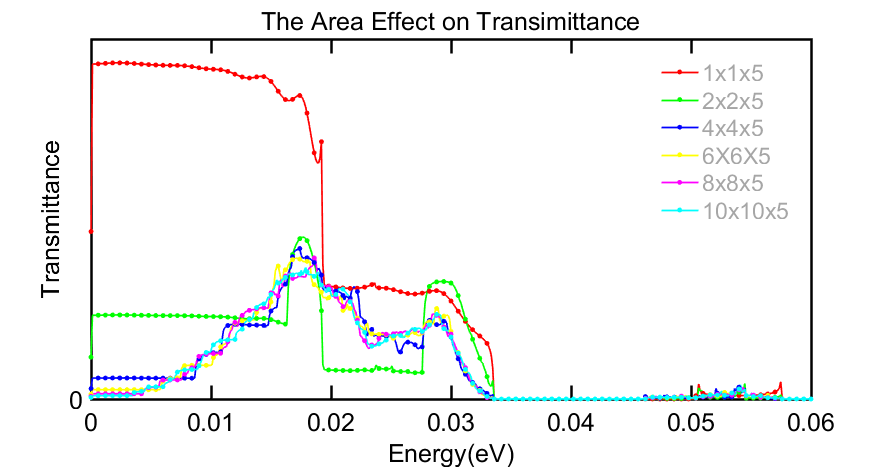
\includegraphics[width=\textwidth]{GaPGaAs_Big.png}
\caption{GaP/GaAs(a)(Colored online)}
\label{fig:Gaa}
\end{minipage}%
\begin{minipage}[t]{0.5\linewidth}
\centering
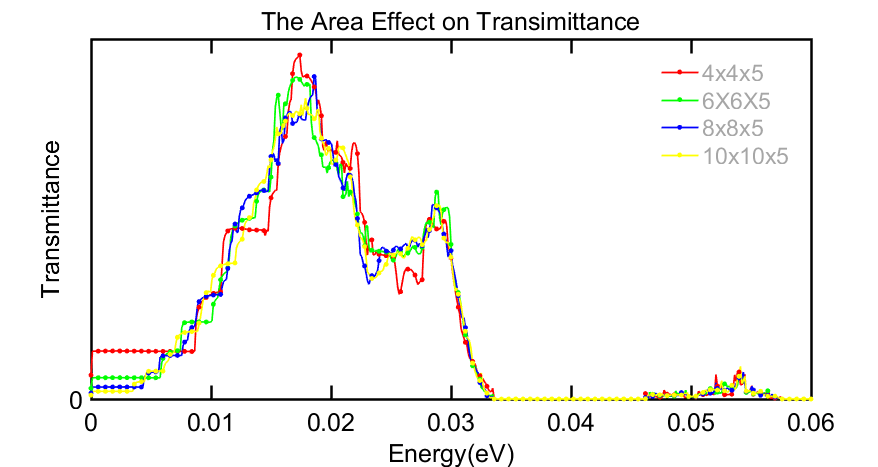
\includegraphics[width=\textwidth]{GaPGaAs_sub.png}
\caption{GaP/GaAs(b)(Colored online)}
\label{fig:Gab}
\end{minipage}
\end{figure}
\par
\hspace{-0.2in}
\begin{figure}
\begin{minipage}[t]{0.5\linewidth}
\centering
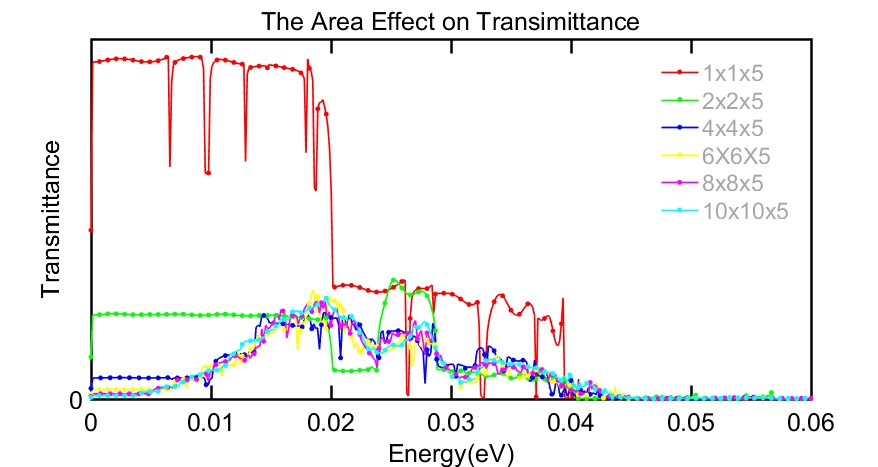
\includegraphics[width=\textwidth]{SiGe_Big.png}
\caption{Si/Ge(a)(Colored online)}
\label{fig:SiGea}
\end{minipage}%
\begin{minipage}[t]{0.5\linewidth}
\centering
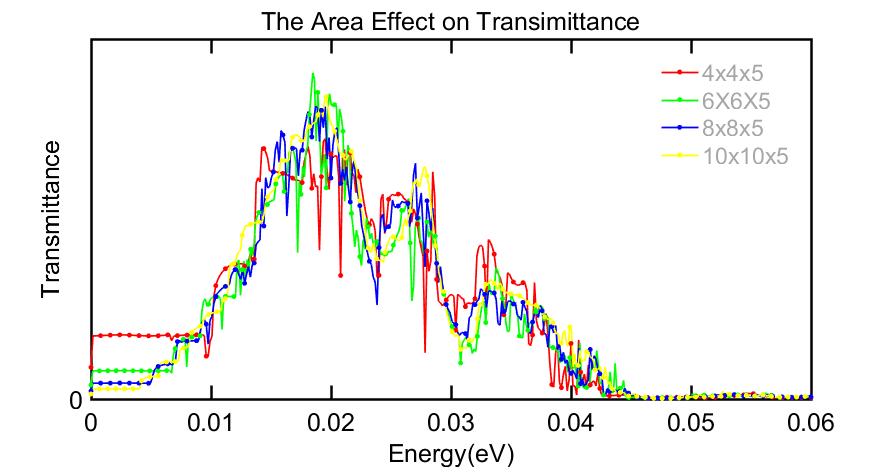
\includegraphics[width=\textwidth]{SiGe_sub.png}
\caption{Si/Ge(b)(Colored online)}
\label{fig:SiGeb}
\end{minipage}
\end{figure}
\subsection{The Optimization of Interface and Device}
After we construct a interface and then get a device for AGF calculation, the first thing we should do is to relax the configuration to lower its total energy. We give a detailed description of the optimization methods we adopt in  \textbf{Appendix C}, and here we will give the example of the optimization of GaN/GaP interface.\\
\indent The crystal structure of GaN is Wurtzite, while the GaP is Zincblende type. Considering that they have the different types of crystal structures, it is a perfect example to explain the optimization process.\\
\indent As shown in the Fig(\ref{fig:centralop}) and Fig(\ref{fig:1DMINop}), the total energy of the whole system becomes lowers as the iteration steps grow and the stress also becomes stable.
\begin{figure}
\begin{minipage}[t]{0.5\linewidth}
\centering
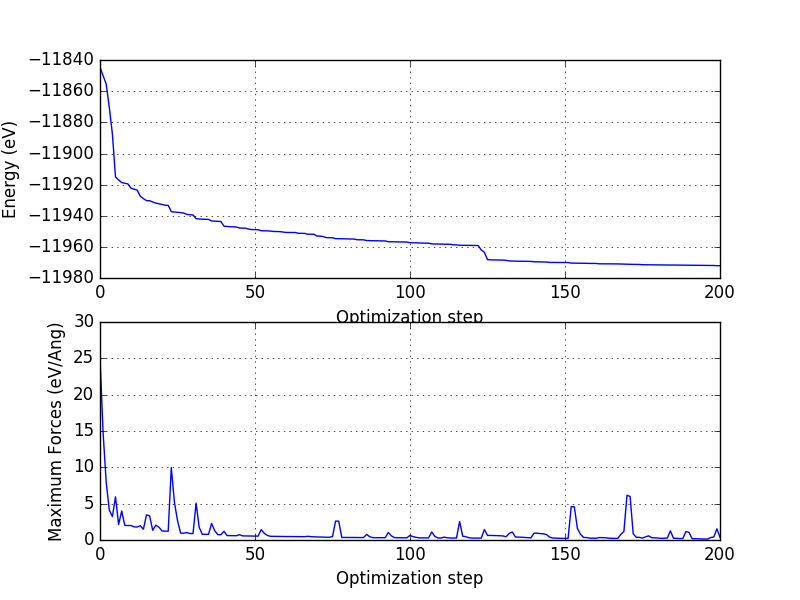
\includegraphics[width=\textwidth]{central.png}
\caption{The central region optimization with rigid ends}
\label{fig:centralop}
\end{minipage}%
\begin{minipage}[t]{0.5\linewidth}
\centering
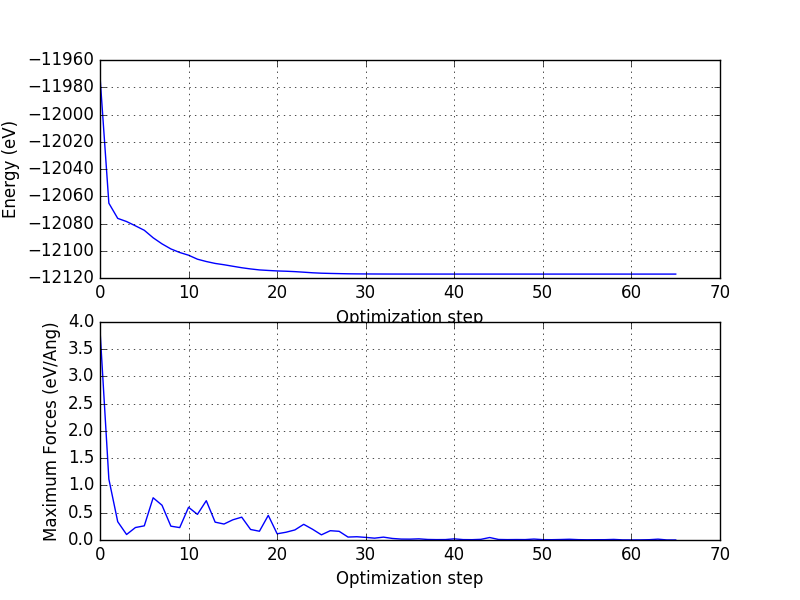
\includegraphics[width=\textwidth]{1DMIN.png}
\caption{1DMIN of the whole device}
\label{fig:1DMINop}
\end{minipage}
\end{figure}

\subsubsection*{The layers of interface}
We use rigid constraints at both ends so the layers of atoms in the interface region can have an effect on the result. We test the different layers of atoms with Si/SiC and it can be clearly shown in Fig(\ref{fig:length1}) and Fig(\ref{fig:length2}), the result becomes consistent when layers are thick enough, so we use four layers in our calculations.
\begin{figure}
\begin{minipage}[t]{0.5\linewidth}
\centering
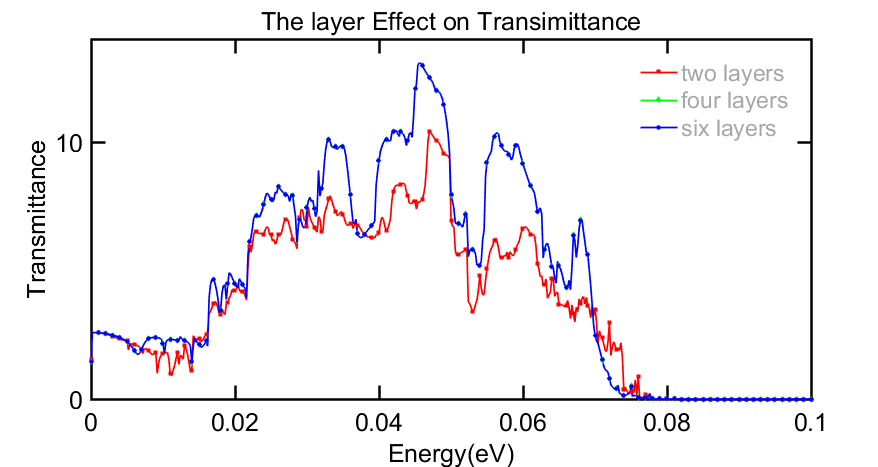
\includegraphics[width=\textwidth]{length1.png}
\caption{Si/Sic (Colored online)}
\label{fig:length1}
\end{minipage}%
\begin{minipage}[t]{0.5\linewidth}
\centering
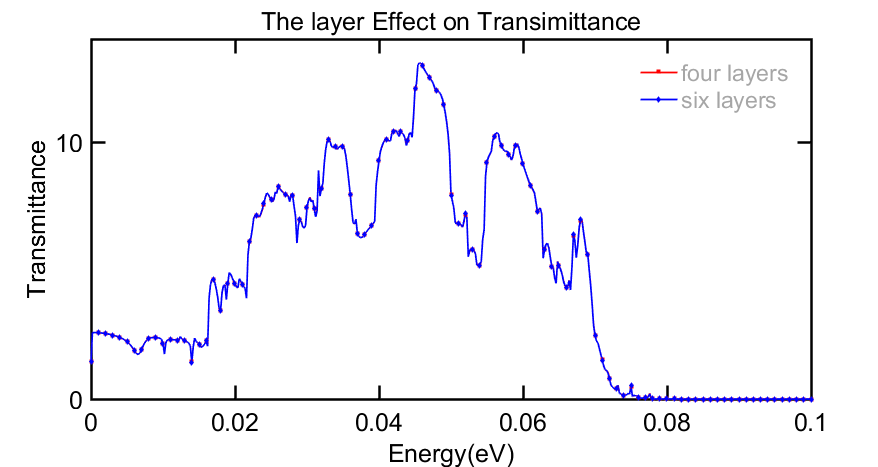
\includegraphics[width=\textwidth]{length2.png}
\caption{Si/SiC interface(four and six)(Colored online)}
\label{fig:length2}
\end{minipage}
\end{figure}
\subsection{Calculation Details}
As we have discussed in \textbf{3.2}, for AFG calculation, the input is the configuration information(the type and the initial position of atoms) and the interaction. The former can be given after we get the device configuration(after optimization), and the former we need define the interaction potential or give from first principle or others. \\
\indent We choose the Tersoff potential given by blabla in our AGF work. The details and a brief introduction to Tersoff potential is in\textbf{Appendix C}. Here we will give the reason why we choose the empirical potential instead of the first principle method:
\begin{itemize}
\item The Tersoff type potential\cite{TeroffIIIV} we use is specifically set for the III-V seimi-conductors and has been proved effective in several works\cite{tersoffwork1,tersoffwork2,teroffwork3,tersoffwork4}.
\item Although several improvements have been made in first principle calculations, the simulation of a system like ours can still be very time-consuming. Just use $Si/SiO^2$ for example, if we use empirical potential to optimize the device it usually cost less than a minute while for first principle calculation it can cost more than a hour if both run on a PC. And that is just the optimization process so even though we use
parallel computing, the first principle cannot been acceptable.
\end{itemize}
\subsubsection*{The bandstructure and the Phonon Density of States(DOS)}
Before we begin to analyze our AGF results, it is essential  to calculate the phonon bandstructure and Density of States, which can inspire our late insight on AGF results.

\begin{figure}

\centering
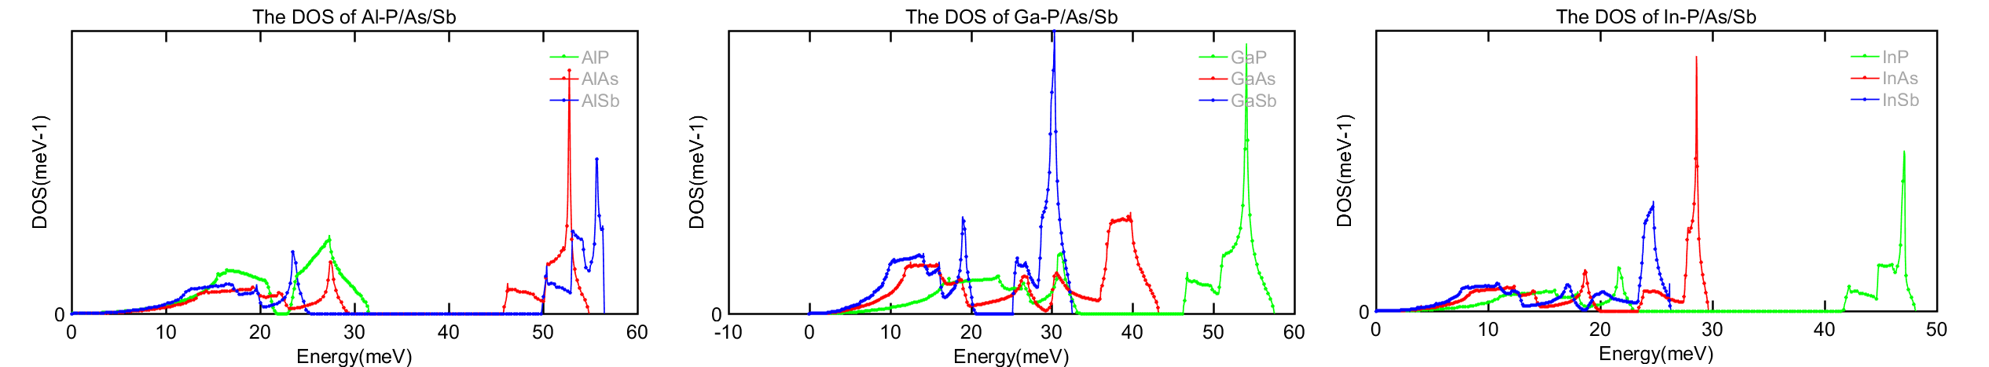
\includegraphics[width=\textwidth]{dos.png}
\caption{DOS(Colored online)}
\label{fig:dosall}
\end{figure}

\subsection{Results}
In real materials, the lattice constants
of the materials across interfaces are often different, and
lattice mismatch could result in atomic reconstruction in
the interfacial region. Such interfacial reconstruction can
change the phonon transmission at the interface and thus
the interfacial thermal conductance. In most of the past works, this effect is ignored but in our work we exploit a relaxation way to cope with this effect.\\
\indent In this section, phonon transmission across a single interface between two semi-infinite III-V semi-conductors as shown in Fig(\ref{fig:TAlP},\ref{fig:TAlAs},\ref{fig:TAlSb}) is studied. As we studied 9 types of III-V semi-conductors in all, so the combinations can be 36, we just show part of the results(Transmittance of AlX(X=P,As,Sb), for example.).

\begin{figure}
\centering
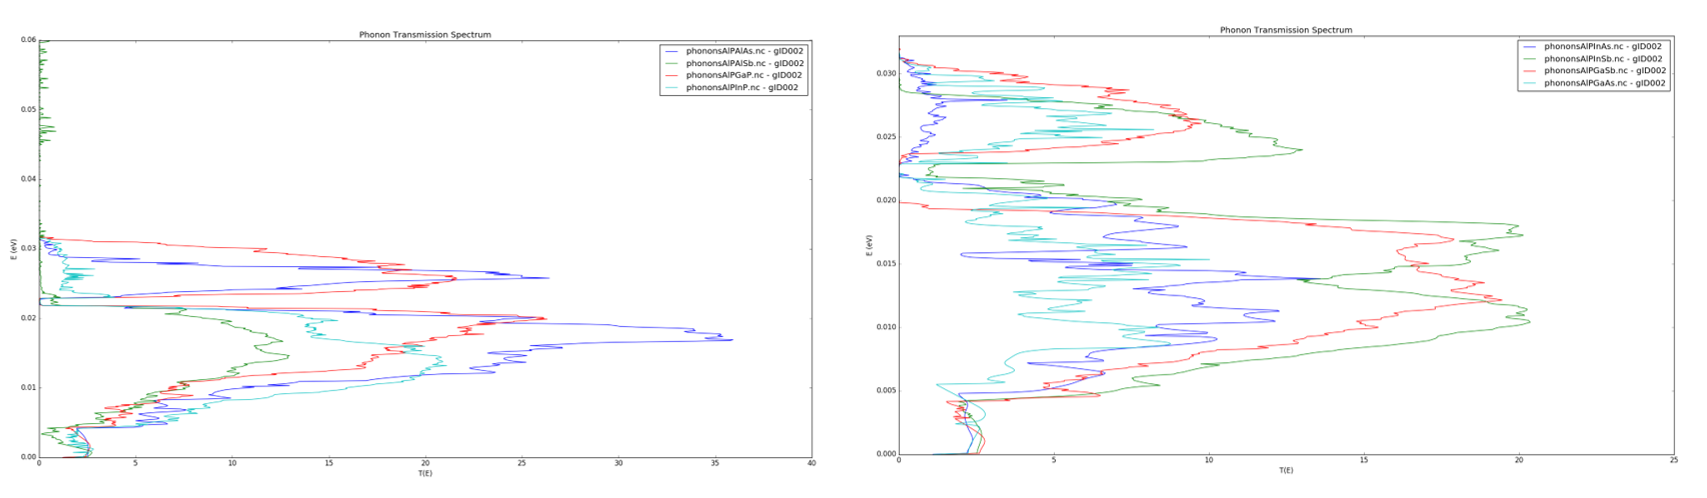
\includegraphics[width=\textwidth]{AlP.png}
\caption{Phonon transmission across a single interface of bulk AlP and other materials(Colored online)}
\label{fig:TAlP}
\end{figure}

\begin{figure}

\centering
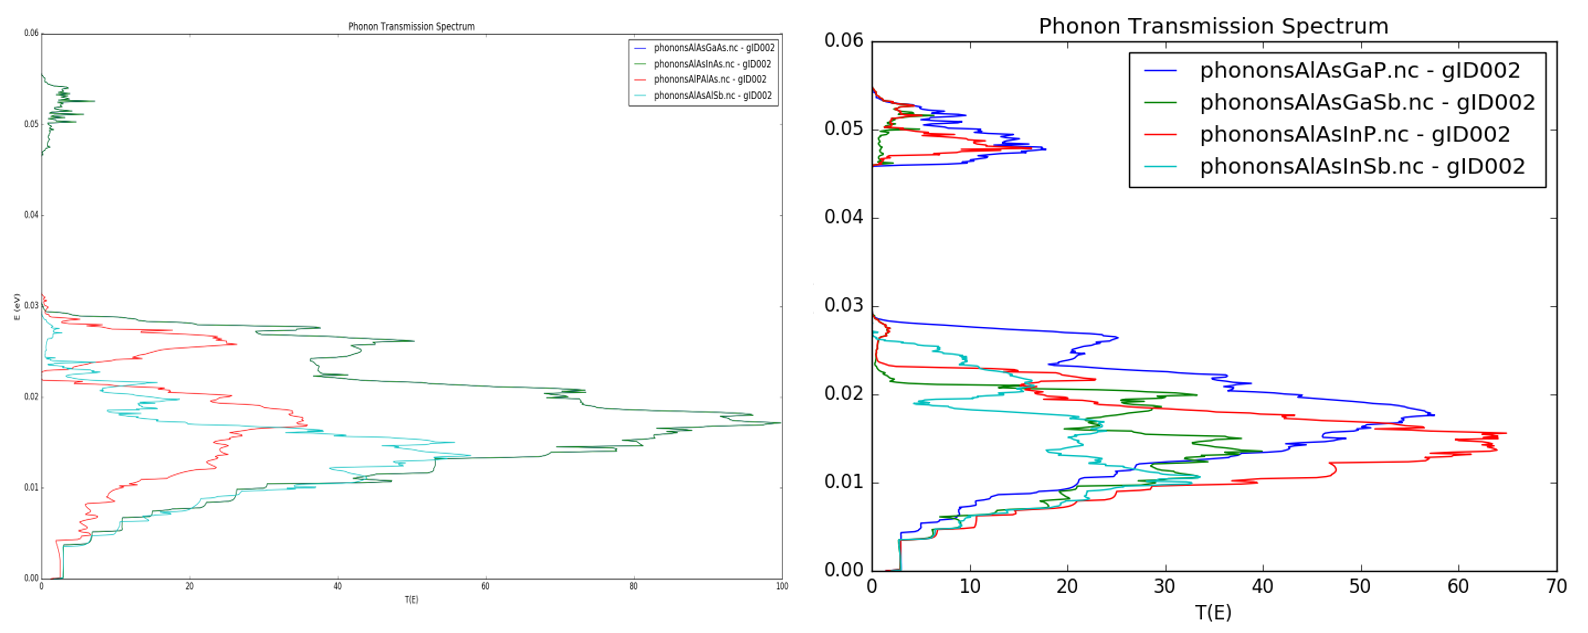
\includegraphics[width=\textwidth]{AlAs.png}
\caption{Phonon transmission across a single interface of bulk AlAs and other materials(Colored online)}
\label{fig:TAlAs}
\end{figure}%

\begin{figure}

\centering
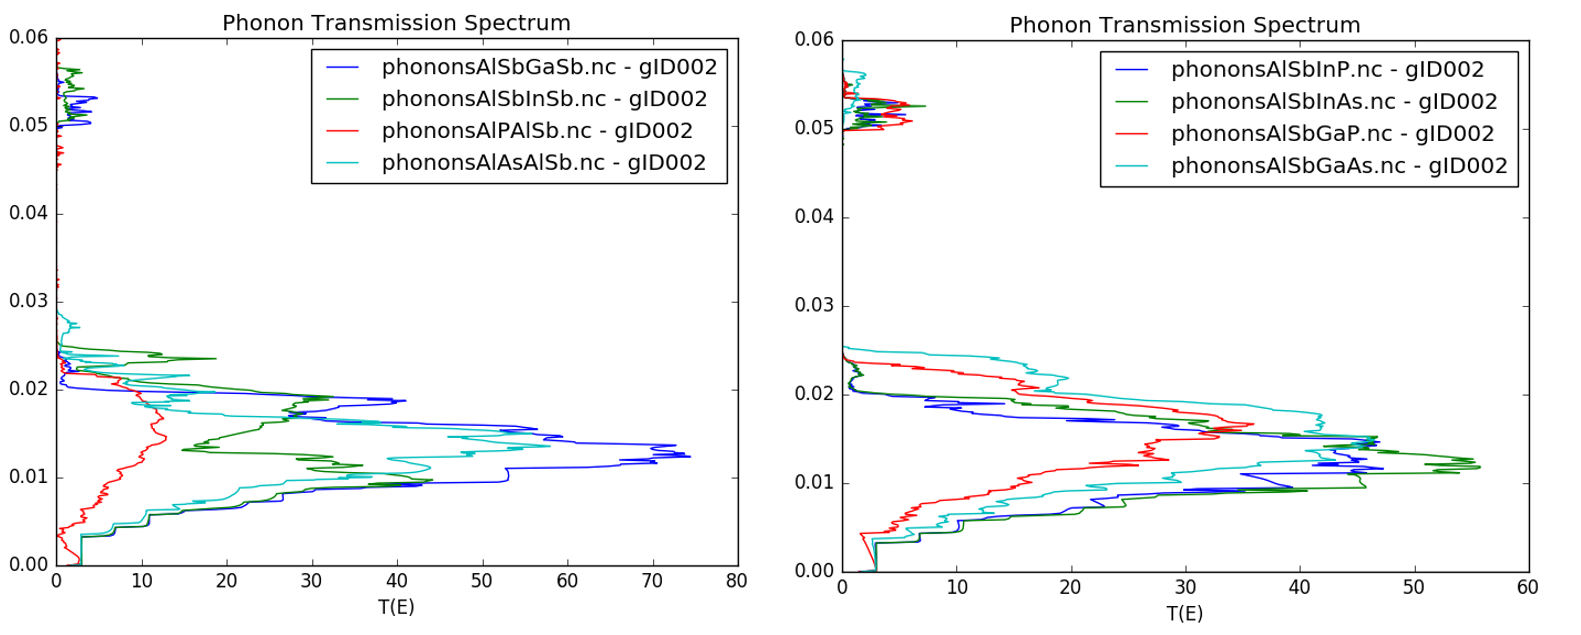
\includegraphics[width=\textwidth]{AlSb.png}
\caption{Phonon transmission across a single interface of bulk AlSb and other materials(Colored online)}
\label{fig:TAlSb}
\end{figure}%

\subsection{Discussion}
We studied the phonon transmission across GaP/GaAs, GaP/GaSb and GaAs/GaSb for example, and the results are shown in Fig(\ref{fig:TGa}). In the low frequency region, there are more similarity with GaP and GaAs in dos, so the transmittance is large while in the high frequency region, the bigger difference in dos caused a low transmittance. And also when the atoms become bigger(heavier), the peak of transmission goes to the lower frequency region, which may be explained by the dominating phonons(having the main percent of energy) change.\\
\indent Here we just give a short and brief discussion of this issue, and we will return to this topic in the later Chapter and also this will be the core focus of our later work.

\begin{figure}

\centering
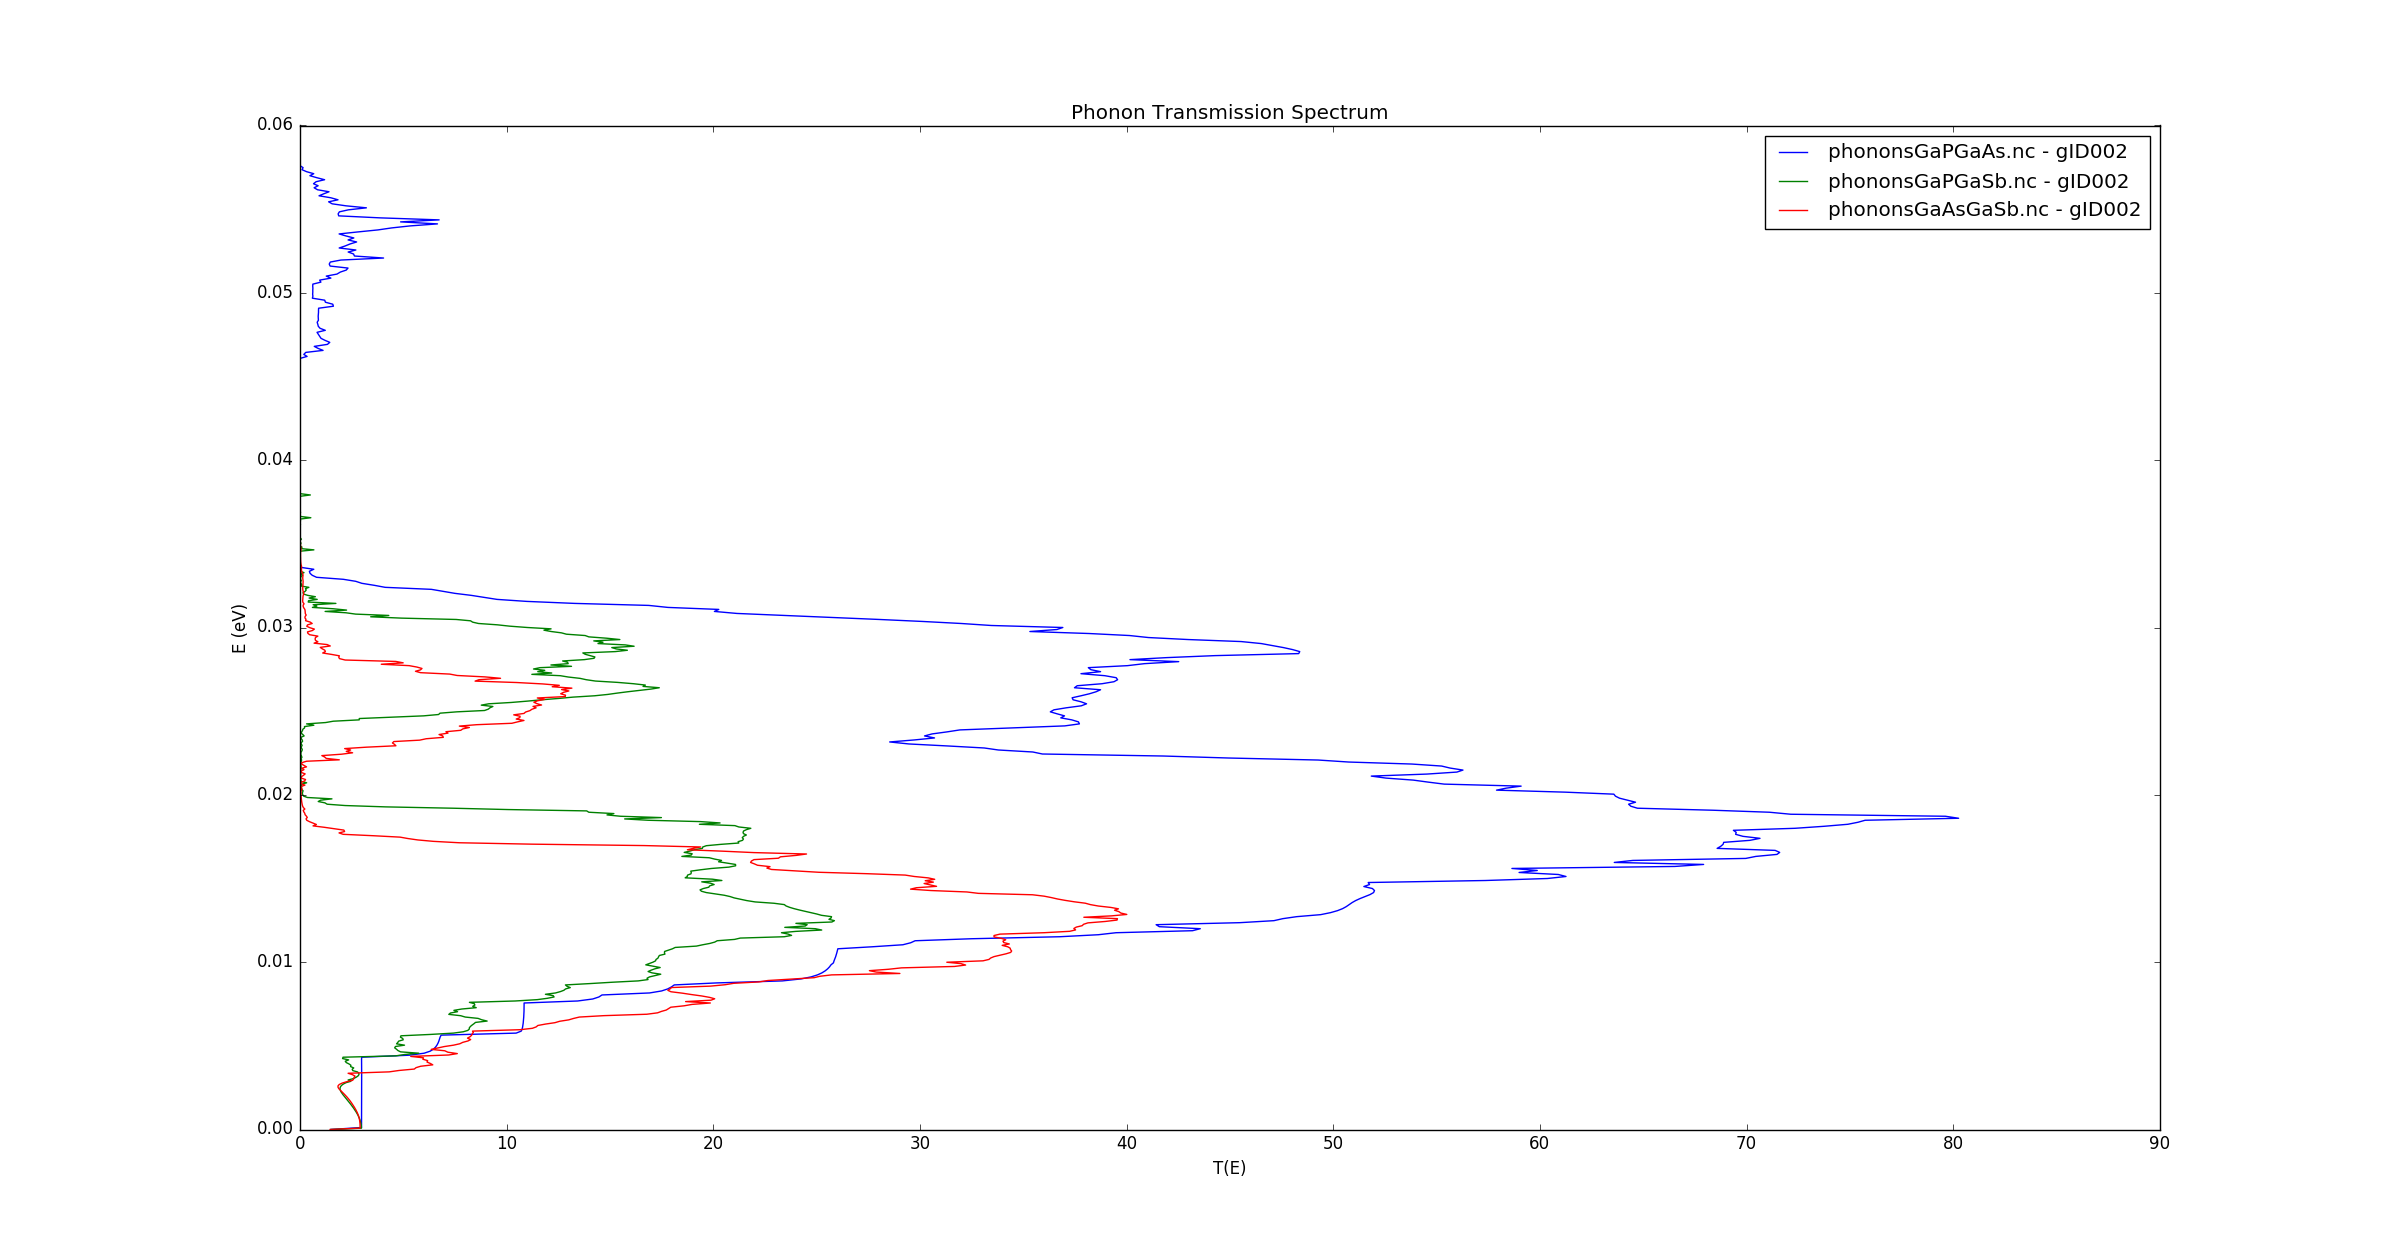
\includegraphics[width=\textwidth]{TGa.png}
\caption{Phonon transmission across a single interface of bulk GaP,GaAs and GaSb(Colored online)}
\label{fig:TGa}
\end{figure}%

\nomenclature{g}{uncoupled green's function matrix}%
\nomenclature{G}{green's function matrix}%
\nomenclature{$\hbar$}{reduced Planck constant(=$h/2\pi$)}%
\nomenclature{\textbf{H}}{harmonic matrix}%
\nomenclature{i}{unitary imaginary number}%
\nomenclature{\textbf{I}}{identity matrix}%
\nomenclature{J}{energy flux}%
\nomenclature{$k_B$}{Boltzmann constant(=1.38 $\times$ $10^{-23}$ kg/$s^2$k)}%
\nomenclature{M}{atomic mass}%
\nomenclature{S}{source matrix}%
\nomenclature{t}{time}%
\nomenclature{i}{unitary imaginary number}%
\nomenclature{A}{matrix for convenience}%
\nomenclature{$\Gamma$}{matrix for convenience}%
\nomenclature{$\tilde{u}$}{column vector consisting of vibrational degrees of freedom}%
\nomenclature{U}{interatomic potential}%
\nomenclature{$\delta$}{a small number corresponding to phonon energy dissipation in contacts}%
\nomenclature{$\sigma$}{thermal conductance (W/K)}%
\nomenclature{$\omega$}{angular frequency(rad/s)}%
\nomenclature{$\sum$}{self-energy matrix}%
\nomenclature{$\tau$}{matrix representing interactions}%
\nomenclature{$\phi$}{column vector representing vibrational degrees of freedom in either contact}%
\nomenclature{$\chi$}{column vector representing the change to the original vector $\phi^R$ after contacts and the device are connected}%
\nomenclature{$\psi$}{column vector representing vibrational degrees of freedom in the connected device}%







 
\nomenclature{LCB}{left contact bulk region}%
\nomenclature{LC}{left contact region}%
\nomenclature{LD}{left device region}%
\nomenclature{RCB}{right contact bulk region}%
\nomenclature{RC}{right contact region}%
\nomenclature{RD}{right device region}%
\nomenclature{d}{device region including LD,RD and D}%
\nomenclature{m}{degree of freedom running index}% 
\nomenclature{p}{matrix row index, or the index of a degree of freedom}%
\nomenclature{q}{matrix row index, or the index of a degree of freedom}%
\nomenclature{R}{disconnected state}%
\nomenclature{*}{complex conjugate of a matrix}%
\nomenclature{$\dag$}{conjugate transpose of a matrix}%
\printnomenclature   %%% 出现的地方
 



\clearpage

%!TEX root = ../thesis.tex
%*******************************************************************************
%*********************************** First Chapter *****************************
%*******************************************************************************

\chapter{Further studies: Do the Optimization and find more underlying physics}  %Title of the First Chapter

\graphicspath{{Chapter4/}}


%********************************** %First Section  **************************************
\setlength{\epigraphwidth}{0.6\textwidth}
\epigraph{“I first heard of this when Fowler was explaining it to one of Rutherford’s closest collaborators, who said ‘very interesting’ in a tone which implied that he was not interested at all. Neither was I.”}
{\textit{Nevil Mott, recollecting the glorious moment he first learned of the difference between metals and insulators.}}
\section[The Bayesian Optimization on ITC]{Designing Nanostructures for Phonon Transport via Bayesian Optimization}
\textit{Thermal boundary resistance (TBR) is a key property for the thermal management of high power
micro- and opto-electronic devices and for the development of high efficiency thermal barrier coatings
and thermoelectric materials. Prediction of TBR is important for guiding the discovery of interfaces
with very low or very high TBR. Based on our study on phonon transmittance between III-V semi-conductors interfaces, we report the prediction of TBR by the machine learning method, our main method is the Bayesian Optimization which also includes the Gussian process regression. The application of this method has been proved efficient in work\cite{ueno2016combo}, and our work is also based on this work and the open code available at \url{https://github.com/tsudalab/combo}. }\\
\textit{We demonstrate optimization of thermal conductance across nanostructures by developing a method combining atomistic Green's function and Baysian optimization. With an aim to minimize and maximize the interfacial thermal conductance(ITC) across four types of III-V semi-conductors(AlP,AlAs,GaP,GaAs) superlattices, the method identifies the optimal structures from calculations of only a few percent of the entire candidates(over $4^6$ structures). The obtained optimal interfacial structures are nonintutive and impacting. The work shows the effectiveness and advantages of material informatics in designing nanostructures to control heat conduction, which can also be extended to other nanostructures and properties\cite{ju2017designing}.}
\subsection{Introduction}
During the past decade, informatics has been successfully applied in many aspects\cite{rajan2015materials,agrawal2016perspective}, namely the integration of
material property calculations or measurements and informatics to accelerate the material discovery and design. In the field of heat transfer, materials informatics has been applied to search for thermalelectric material with low thermal conductivity\cite{carrete2014finding}. However, the nanostructure optimization for thermal transport, especially in multi-structures is still in its infancy. In this work, we use the Bayesian optimization methods based on our former atomistic Green's function(AGF) method to identify the interficial strutures that realize maximum and minimum ITC.
\subsection{Methodolody}
%%%%%%%%%%%%%%%%%%%%%%%%%%%%%%%%%%%%%%%%%%%%%%%%%%%5
\begin{figure}

\centering
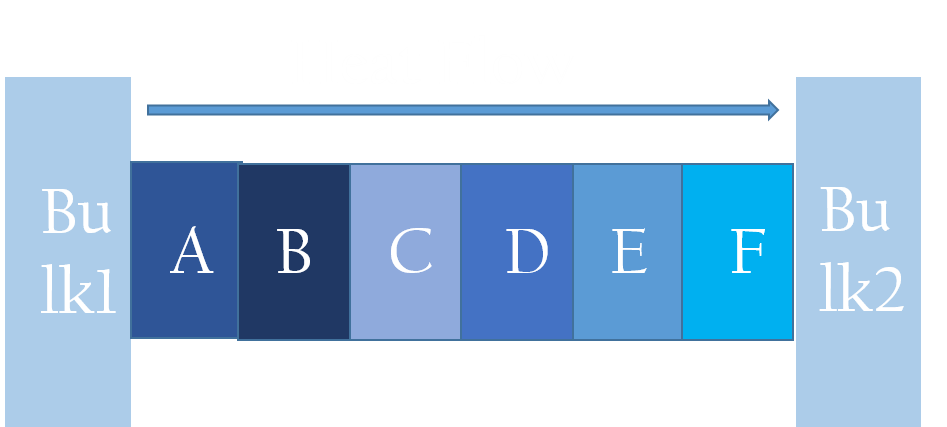
\includegraphics[width=0.5\textwidth]{device.png}
\caption{The illustration of the structure we study}
\label{fig:agfdevice}
\end{figure}
\begin{figure}
\centering
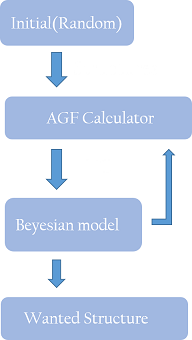
\includegraphics[height=8cm]{map.png}
\caption{Schematics of the materials informatics method combing the atomistic Green function (AGF) and Bayesian optimization}
\label{fig:agfmap}

\end{figure}
%%%%%%%%%%%%%%%%%%%%%%%%%%%%%%%%%%%%%%%%%%%%%%%%%%%%%
We explain the method by taking a problem to design the superlattice interfacial strcuture to tune the heat conduction across the interface between AlP, AlAs, GaP and GaAs. As illustrated in Fig(\ref{fig:agfdevice}), the system consists of an interfacial region between two materials A(AlP) and B(AlP) with infinite thickness. For the convinience of calculation, the lattice mismatch between these four materials is ignored because this effect has been included in our former study in Chapter 3.
The interfacial structure is divided into six parts, each of which can consist of AlP,AlAs,GaP or GaAs, and the optimization problem is how to arrange the Si and Ge atoms to obtain the largest and the smallest ITC.\\
\indent Four basic elements are required when conducting
material informatics: the descriptor, evaluator, calculator,
and optimization method. The descriptors are used to
describe the possible structure candidates considered during the optimization. 
In this study, we use several ints to
describe the state of each atom: “1”,“2”,“3” and “4” represent the
AlP,AlAs,GaP and GaAs atom, respectively. As for the evaluator, the value
of ITC is chosen to quantitatively evaluate the performance
of each configuration.\\
\indent Because we have given the explicit form of AGF method in form Chapter, now we just give a breif introduction of the Bayesian Optimization method.Actually, we are interested in solving that a problem:
\begin{equation*}
x^{*}=arg min_x f(x)
\end{equation*}
Under the constraints that
\begin{itemize}
	\item $f$ is a black box for which no closed form is know(nor its gradients)
	\item $f$ is expensive to evaluate
	\item And evaluation of $y=f(x)$ may be noisy
\end{itemize}
Under these conditions, it is quite nice to employ the Bayesian optimization method. Below is a standard Bayesian optimization loop\cite{snoek2012practical}:\\
For $t=1:T$:
\begin{enumerate}
	\item Given observations $(x_i,y_i=f(x_i))$ for $i=1:t$, build a probabilistic model for the objective $f$. Itegrate out all possible true functions, using Gaussian process regression\cite{rasmussen2006gaussian}. 
	\item Optimize a cheap acquisition/utility function $\mu$ based on the posterior distribution for sampling the next point
	\begin{equation*}
	x_{t+1}=arg min_x \mu(x)
	\end{equation*}
	Exploit uncertainty to balance exploration against exploitation.
	\item Sample the next observation $y_{t+1}$ at $x_{t+1}$
\end{enumerate}
Then comes the core of this method: Acquisition functions\cite{brochu2010tutorial}.Acquisition functions $\mu(x)$ specify which sample $x$ should be tried next
\begin{itemize}
	\item Expected improvement(default): $-EI(x)=-\mathbb{E}[f(x)-f(x^{+}_t)]$
	\item Lower confidence bound: $LCB(x)=\mu_{GB}(x)+\kappa \sigma_{GP}(x)$
	\item Probaility of improvement: $-PI(x)=-P(f(x) \geq f(x^{+}_t)+\kappa)$
\end{itemize}
where $x^{+}_t$ is the best point observed so far.\\
\indent In our work, we emplot the open-source Bayesian optimization library $\mathcal{COMBO}$\cite{ueno2016combo} to perform the optimization process. Bayesian optimization is an experimental design algorithm based on machine learning\cite{jones2001taxonomy}. As shown in Fig(\ref{fig:agfmap}), suppose that ITCs of $n$ candidates are initially calculated, and we are to choose the next one to calculate. A Bayesian regressio function is learned from $n$ pairs of descriptors and ITCs(training examples). For each of teh remaining candidates, a predictive distribution of ITCs is estimated. The best candidate is choosen based on the criterion of expected improvement\cite{jones2001taxonomy}.Finally, ITC is calculated for the chosen candidate, and it is added to the training examples. By repeating this procedure, the calculation of ITCs is scheduled optimally, and the best candidate can be found quickly.\\
\indent As the prediction model, we exploy a Bayesian linear regression model combine with a random feature map,
\begin{equation}
y=w^{T}\psi(x) +\epsilon
\end{equation}
where $x$ is a d-dimensional vector corresponding to a candidate, $w$ is a D-dimensional weight vector, and $\epsilon$ is the noise subject to normal distribution with mean 0 and variance $\sigma$. The random feature map is chosen so that the inner product corresponds to the Gaussian kernel\cite{rahimi2008random}:
\begin{equation}
\psi(x)^T\psi(x^{'})=exp(-\frac{|x-x^{'}|^2}{\eta^2})
\end{equation}
\indent The performance of the model depends on hyperparameters $\sigma$ and $\eta$. In $\mathcal{COMBO}$, they are initialized according to a heuristic procedure bu Yang $et al.$\cite{yang2015carte}. 
\subsection{Reuslts and Discussion}
In our calculation, the predicted struture with maximum ITC comes to convergence within calculations less than 200 structures, which is only $4.9\%$ of the total number of candidates(4096). In Fig(\ref{fig:maxITC}), we also calculate the structures with no interface to compare with the optimazed structures. It can be clearly seen that almost in all frequencies, the aimed structure(412314) has very low transmittance. For phonon energy in the central region(0.015eV-0.025eV), the wave-length of phonons is almost the same as the length of unit cell so that the transmissions of different strutures can be very similar. On the other hand, in other regions, the transmission function strongly depends on the strcuture.
\begin{figure}
\centering
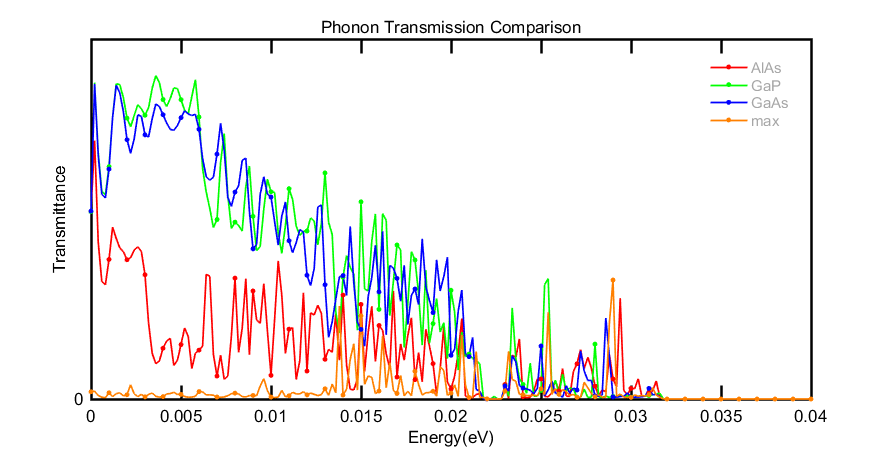
\includegraphics[width=0.8\textwidth]{max.png}
\caption{The illustration of the structure we study}
\label{fig:maxITC}
\end{figure}\\
\indent Now that the optimal struture is identified, we can move on  to look into the mechanisms behind the big ITC. And this is actually the goal of the next work, and for this topic here, there are mainly below ways to discuss:
\begin{enumerate}
	\item The first
obvious attempt is to see it from the view of phonon
dispersion relations and phonon density of states (DOS), as
is broadly done to discuss phonon interference.
	\item Then to gain a deeper understanding of the physics of
phonon transport in the optimized structure, we can look into
the role of phonon coherence, which can cause constructive
and destructive interferences.
\end{enumerate}
\subsection{Conclusions}
In conclusion, we identify the III-V semi-conductors composite interfacial structures that maximize the ITC across two contacts by the developed framework combining the atomistic Green function and Bayesian optimization methods.The optimal structures are obtained
by calculating only a few percent of the total candidate
structures, considerably saving computational resources. And this work not only gives a practical example to design the thermal nanostructures with desired thermal properties(i.e. ITC), but also leaves us an entrance to further study on the physics behind the data.\\

\setlength{\epigraphwidth}{0.6\textwidth}
\epigraph{“The work using machine learning tool such as Bayesian optimization is quite great, but when you get the final result you still don't know why the result should be like this... You know, regression, may data back to Newton's age, but you can use this to discover real science.”}
{\textit{Junichiro Shiomi(Professor, Univeristy of Tokyo)}}
\section[Figure out the physics]{Study on the factors affecting the ITC and Phonon tramsmittance}

\subsection{Mechanism behind the phonon interface transmittance}
As we have calculated and given primary dicussion in former chapter, we gain the phonon transmittance of total combinations of III-V semi-conductors using AGF method. And we also further use the Bayesian optimization method to get the desired strusture with maximum(or minumum) ITC, our next work will focus on the physcis behing these data, namely:
\begin{itemize}
	\item Find out the factors that affect the transmittance and also the way how they take effect. Then try to establish the new model not just following the old AMM or DMM pattern.
	\item Based on the former work, find out a predictor model to derive the desired structure by the knowledge of physics.
\end{itemize}
\subsection{Regression Analysis}
Actually, there have been several attempts on that issue these years, and the most recent one is the paper\cite{zhan2017prediction} published on Nature Scientific Report in June, 2017. In this work, they combine the past data gained from many past works and try to find out a model to predict the TBR(thermal boundary
resistance). As shown in Fig(\ref{fig:TBR}),the descriptors used for the AMM and DMM predictions are temperature, density, speed of sound (longitudinal and transverse), and unit cell volume, which we defne as “AMM and DMM descriptors”. However, they didn't 'jump out' the famework of AMM and DMM and they only consider the bulk properties so that their work is far from reaching the true physics behind this issue. 
\begin{figure}
\centering
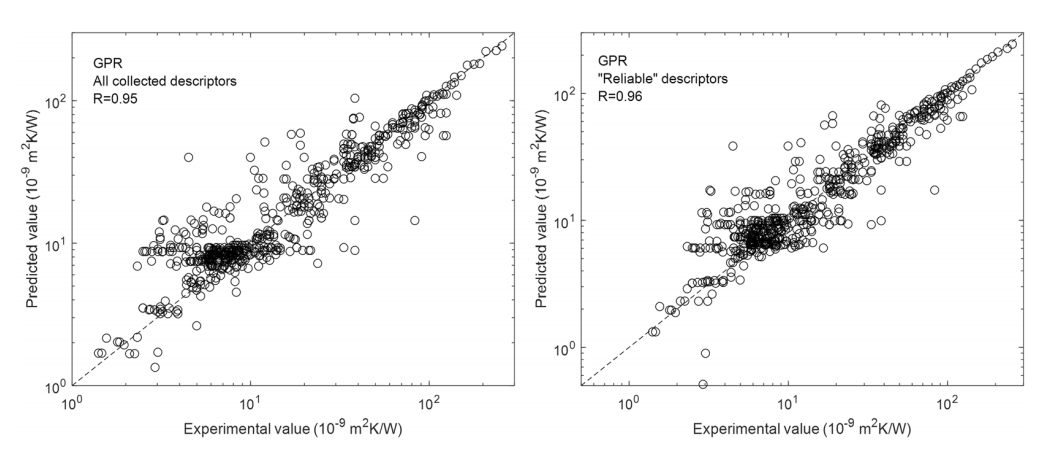
\includegraphics[width=0.8\textwidth]{TBR.png}
\caption{Correlation between the experimental values and the values predicted by the GPR model using the
“reliable” descriptors and all collected descriptors\cite{zhan2017prediction}.}
\label{fig:TBR}
\end{figure}\\
\indent Actually, motivated by a recent work\cite{hua2017slip} on Slip Boundary Conditions in Ballistic–Diffusive Heat Transport, the MFP of phonon is thought to play an important role in phonon interface transmittance. Now we have stepped forward to consider more factors based on derivation of BTE or other experiments to do the regression, and this is the heart of the later work.\\

\textbf{My code of the AGF method and the Bayesian optimization is available at \url{https://github.com/chieko-feiyuxiao/Oric}}
%%!TEX root = ../thesis.tex
%*******************************************************************************
%*********************************** First Chapter *****************************
%*******************************************************************************

\chapter[Figure out the physics: the regression method]{The study on the factors affecting the ITC and Phonon tramsmittcance}  %Title of the First Chapter

\graphicspath{{Chapter5/}}


%********************************** %First Section  **************************************

Regression
%\include{Chapter6/chapter6}
%\include{Chapter7/chapter7}



% ********************************** Back Matter *******************************
% Backmatter should be commented out, if you are using appendices after References
%\backmatter

% ********************************** Bibliography ******************************
\begin{spacing}{0.9}

% To use the conventional natbib style referencing
% Bibliography style previews: http://nodonn.tipido.net/bibstyle.php
% Reference styles: http://sites.stat.psu.edu/~surajit/present/bib.htm

\bibliographystyle{apalike}
%\bibliographystyle{unsrt} % Use for unsorted references
%\bibliographystyle{plainnat} % use this to have URLs listed in References
\cleardoublepage
\bibliography{References/references} % Path to your References.bib file


% If you would like to use BibLaTeX for your references, pass `custombib' as
% an option in the document class. The location of 'reference.bib' should be
% specified in the preamble.tex file in the custombib section.
% Comment out the lines related to natbib above and uncomment the following line.

%\printbibliography[heading=bibintoc, title={References}]


\end{spacing}

% ********************************** Appendices ********************************

\begin{appendices} % Using appendices environment for more functunality

%!TEX root = ../thesis.tex
% ******************************* Thesis Appendix B ********************************
\graphicspath{{Appendix1/}}
\chapter{Frequency-dependent MC Method}
\section*{Introduction}
Actually, a typical MC simulation strategy for phonon transport is relatively the same as what we used in our MC simulation:we initialize, launch, and trace phonon
ensembles in terms of temperature, frequency, polarization, and
positions. Local temperature distribution varies depending on the
positions of these ensembles.Typically, because there we will take abut the simulation considering dispersion and polarization, which results in the different treatment in phonon scattering mainly.
The simulation starts by initializing all the
phonon ensembles (including those to be launched from the constant-
temperature boundary and within the material due to heat
generation at each $\Delta$t). These ensembles are moved ballistically
from one position to another within the time interval of $\Delta$t, assuming
that ensemble properties remain unaltered. Ensembles that hit
a constant-temperature boundary are recorded in terms of energy
for heat flux calculation and then deleted. Those that encounter an
insulated surface are assumed to be reflected specularly or diffusively.
Otherwise, ensembles reside at the corresponding locations
after the ballistic movement.Once the propagation phase is complete,
local temperature distribution is calculated based on the
positions of the ensembles. It is important to notice that local phonon
distribution function after the propagation phase is different
from the equilibrium distribution (i.e., the Bose–Einstein distribution).Only the local distribution of total phonon energy is known.
Although a medium can still be in a non-equilibrium state, it is
possible to calculate ‘pseudo-temperature’ distribution\cite{BTE1} assuming
that equilibrium exists.\\
 Next, we will give a introduction to frequency-dependent MC based on Wong's work\cite{wongMC}.
\section*{Method}
\subsection*{Phonon descriptions - dispersion relation, density of states, and group velocity}
The data points of the dispersion relation for silicon are provided
by Brockhouse\cite{brockhouse}.And Wong gives quadratic expressions to fit the dispersion data.Thus,calculating
the angular frequency with known wave vector or vice versa can
be achieved easily during a MC simulation. 
\begin{figure}[htbp!] 
\centering    
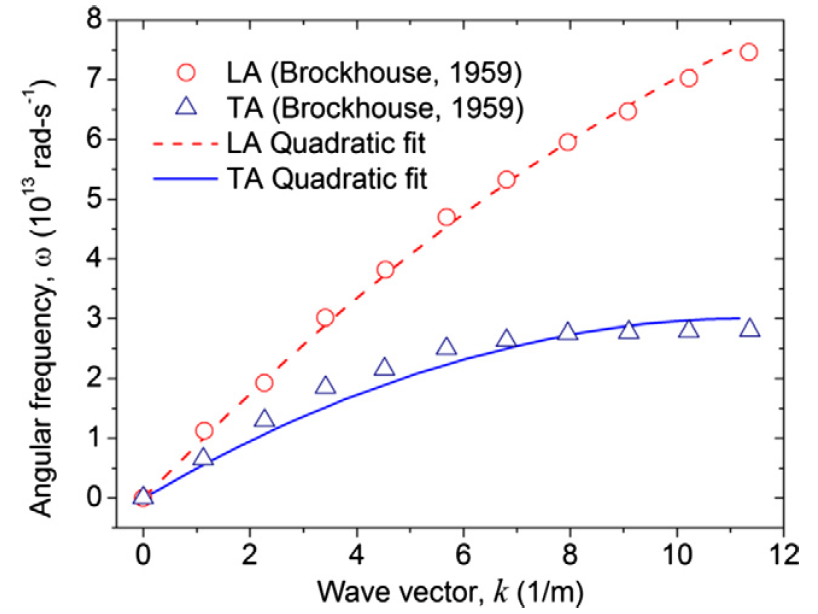
\includegraphics[width=0.6\textwidth]{dispersion}
\caption[Phonon Dispersion of Silicon]{Data points of the dispersion relation of silicon obtained from Brockhouse\cite{brockhouse}.}
\label{fig:dispersion}
\end{figure}
\indent And the quadratic expressions
for the LA- and TA-dispersion relations are obtained as:
\begin{equation}
\omega=9280k - 2.234 \times 10^{-7} k^2 (LA) \label{con:1}
\end{equation}
\begin{equation}
\omega= 5240k - 2.278 \times  10^{-7} k^2 (TA) \label{con:2}
\end{equation}
When the dispersion relation is known, the phonon density of states for a given polarization branch, $D(\omega,p)$, is calculated as:
\begin{equation}
D(\omega ,p)=\frac{k^2}{2 \pi v_g(\omega,p)}
\end{equation}
And the group velocity of the phonon, $v_g(\omega,p)$ can be calculated as:
\begin{equation}
v_g(\omega,p)=\frac{\partial \omega}{\partial k}   \label{con:4}
\end{equation}
\subsection*{Determining properties of phonon ensembles – quantity,
frequency, velocity, and polarization}
To start a MC simulation, the required number of statistical
ensembles needs to be specified and initialized. This is done by
first calculating the total actual number of phonons present in
the medium. Since a ‘‘reference temperature’’ is set in the simulation,
only phonons that are created beyond the reference are initialized.
Therefore, the initial number of phonons available for
carrying excess heat in the medium above the reference is calculated
as:
\begin{equation}
N_{ph,ini}=XYZ \sum_p \sum_i [f_0(\omega_i,T_{ini},p)-f_0(\omega_i,T_{ref},p)]D(p,\omega_i)\Delta \omega_i
\end{equation}
where the index p includes two transverse acoustic (TA) and one
longitudinal acoustic (LA) polarization branches of phonons.
And a scaling
factor, Wscaling, is used to represent the actual number of phonons
that each statistical ensemble carries:
\begin{equation}
W_{scaling}=\frac{N_{ph,ini}}{N_{en,m}}
\end{equation}
where $N_{en,m}$ is the initial number of statistical ensembles used to represent the total actual number of phonons present in the medium. At each time step, $\Delta$, the excess number of phonons emitted from a boundary with constant temperature of $T_R$ or $T_L$ in reference to $T_{ref}$ at each time step is computed as:
\begin{equation}
N_{ph,R}=XY {\Delta t} \sum_p \sum_{i=1}^{N_b}[f_0( \omega_i,T_R)-f_0( \omega_i,T_{ref})][ \vec{v_g}( \omega_i) \times \hat{n}]D( \omega_i,p) \Delta \omega_i
\end{equation}
where $(\vec{v_{\omega,g}} \times \hat{n})$ is the phonon group velocity normal to the boundary. Thus, the scaling factor becomes:
\begin{equation}
W_{scaling}=\frac{N_{ph,R}}{N_{en,R}}
\end{equation}
The next step is to determine the frequency of a phonon ensemble
launched from the $T_R$-boundary. This is done by first constructing
the CPDF of the number of phonons over the frequency spectrum
as:
\begin{equation}
R_i=\sum_{j=1}^i N_j / \sum_{j=1}^{N_b} N_j  \label{con:R}
\end{equation}
where
\begin{equation}
N_j=\Delta \omega _j  \lbrace [f_0(\omega_j,T_R) - f_0(\omega_j,T_{ref})] D(\omega_j, LA) +2 D(\omega_j, TA) \rbrace 
\end{equation}
In Eq(\ref{con:R}), the frequency spectrum is divided into $N_b$ intervals. Then a random number, denoted as $Ran_{\omega}$, si drawn such that:
\begin{equation}
R_{i-1} < Ran_{\omega} < R_i
\end{equation}
and the actual frequency of the statistical ensemble is calculated as:
\begin{equation}
\omega = \omega_i + (2 Ran_{\omega} - 1) \frac{\Delta \omega_i}{2}
\end{equation}
At last, when the frequency of the ensemble is known, we can then determine its polarization bu computing the ratio of the LA-phonons to the total number of phonons n all polarization branches in the $\omega$ interval, which is given as:
\begin{equation}
P_{LA,i}=\frac{[f_0(\omega_i,T_R)-f_0(\omega_i,T-{ref})]D(\omega_i,LA)}{[f_0(\omega_i,T_R)-f_0(\omega_i,T_{ref})][D(\omega_i,LA)+2D(\omega_i,TA)]}
\end{equation}
A random number, $Ran_P$, is then drawn to compare with $P_{LA}$,i. If $Ran_P$
is less than $P_{LA}$,i, then the ensemble belongs to the LA polarization
branch; otherwise, it belongs to the TA polarization branch. The
same procedures are applicable for the $T_L$-boundary. With the frequency
and polarization branch known, the group velocity of the
ensemble can be determined easily using Eqs. (\ref{con:1}), (\ref{con:2}), and (\ref{con:4}).

\subsection*{Sampling initial launching and scattering angles,tracking algorithms}
The same with the MC method we used.
\subsection*{'Pseudo-temperature' calculation}
Once the statistical ensembles of phonons start to propagate
and interchange between small control volumes (or computational
elements) within the entire computation domain, the resultant local
phonon distribution loses its thermodynamic equilibrium. In
order to calculate the local temperature, however, it is necessary
to assume that the total energy carried by ensembles of phonons
in a local computational element is equal to the total phonon energy
computed using the Bose–Einstein distribution for the same
volume. The temperature obtained under such condition is called
as a ‘pseudo-temperature’, denoted as $T_{pseudo}$.Therefore, the following
equation needs to be solved for the $T_{pseudo}$ at each time step:
\begin{equation}
\sum_p \sum_{i=0}^{N_b} \hbar \omega_i [f_0(\omega_i,T_{pseudo})-f_0(\omega_i,T_{ref}]D_i(\omega_i,p) \Delta \omega_i = \frac{E(x,y,z)}{\Delta x \Delta y \Delta z }
\end{equation}
which varies locally.$E(x,y,z)$ is the local energy carried by phonon ensembles within a computational element with $(\Delta x \Delta y \Delta z)$ volume.
\subsection*{Phonon scattering treatment in MC simulation}
Here we go to the most important part. Scattering of phonons consists of two types, following either a
Normal (N) or an Umklapp (U) process\cite{Ashcroft,Ziman,zimanphonons}.
Both processes
tend to restore equilibrium; however, only U-processes resist heat
conduction. In this work, only three-phonon scattering is accounted
during MC simulation although it is probable that fourphonon
scattering and beyond may occur at high temperatures,
which will be left to future studies. In the three-phonon scattering
processes, two phonons can be combined to yield one phonon or a
phonon can be decomposed into two separate phonons. Both Nand
U-processes follow energy conservation as:
\begin{equation}
\hbar \omega_1 + \hbar \omega_2 \leftrightarrow \hbar \omega_3 \label{con:30}
\end{equation}
The indices 1, 2, and 3 indicate three different phonons, respectively,
and the process given in Eq(\ref{con:30}) is reversible.
In addition,
phonon scattering follows momentum conservation. For N-process,
it is given as:
\begin{equation}
k_1 + k_2 \leftrightarrow k_3
\end{equation}
The $k$'s are the wave vectors of phonons. For U-process, it follows that:
\begin{equation}
k_1 + k_2 \leftrightarrow k_3 + G
\end{equation}
where $G$ is the lattice reciprocal vector. Details and physics involved
in phonon scattering will not be further discussed here because
they are covered extensively in any solid state physics books.
\indent In the current MC simulation, the parameter involved to account
for the phonon scattering is the total relaxation time (i.e.,
$\tau-{NU}$), which includes both N- and U-processes. According to the
Mathiessen rule, it is given as\cite{Ashcroft,zimanphonons}:
\begin{equation}
\frac{1}{\tau_{NU}}=\frac{1}{\tau_{N}}+\frac{1}{\tau_{U}}
\end{equation}
Thus, the CPDF of phonon scattering between $t$ and $t + \Delta t$ is written as:
\begin{equation}
R_{scat} = 1- exp (\frac{- \Delta t}{\tau_{NU}})
\end{equation}
In order to determine if a phonon ensemble is scattered after a time
step of $\Delta t$, a random number $Ran_{scat}$ is drawn and compared to $R_{scat}$. If $R_{scat}$ is less than $R_{scat}$, the ensemble is scattered. Hence Hence ensemble
frequency, polarization, and direction are reset. Relaxation times
are typically temperature and frequency dependent; therefore,
these quantities are to be calculated at each time step. For silicon,
these properties are well-documented. Here, we can use the relaxation
times expressions proposed by Holland\cite{hollandanalysis} for three-phonon scattering
and employed by many researchers in MC simulations\cite{monte1,monte2} since these expressions produced good fit for the thermal
conductivity of silicon in different temperature range. The inverse
relaxation times for N- and U-processes are given as follows:
\begin{equation}
LA-phonons \quad  and\quad N or U-process \rightarrow \tau_{LA,NU}^{-1}=B_l \omega^2 T^3
\end{equation}


\begin{equation}
TA-phonons \quad  and\quad N-process \rightarrow \tau_{TA,N}^{-1} =
\begin{cases}
B_T \omega^2 T^4 & \forall \omega < \omega_{1/2}\\
0 & \forall \omega \geq \omega_{1/2}
\end{cases}
\end{equation}

\begin{equation}
TA-phonons\quad  and\quad  U-process \rightarrow \tau_{TA,U}^{-1} =
\begin{cases}
0 & \forall \omega < \omega_{1/2}\\
\frac{B_{TU} \omega^2}{sinh(\hbar \omega / k_B T)} & \forall \omega \geq \omega_{1/2}
\end{cases}
\end{equation}
where $B_L, B_T, and B_{TU}$ are constants to be determined using bulk
thermal conductivity data, and x1/2 is the frequency corresponding
to $k/k_{max}$ = 0.5 based on the $TA-dispersion$ curve. The values of these
constants will be given in the chart\cite{chen2005monte}.\\

\begin{table}[!hbp]
\centering
\begin{tabular}{|c|c|}
\hline $B_T$  &$9.3 \times 10^{-13}$ \\
\hline $B_L$ &  $1.0 \times 10^{-30} (deg^{-3}s)$ \\
\hline $B_{TU}$&$5.50 \times 10^{-18} s$\\
\hline    
\end{tabular}\\
\caption{B parameters}
\end{table}

\noindent During the process of phonon scattering, the frequency/energy
of each scattered phonon ensemble is reset while additional energy
may be added or removed. Thus it is crucial to include an additional
step to counteract this imbalance of energy within a control
volume. A destruction/creation scheme for phonons can be implemented
to prevent any excess energy gain or loss, and the added/
deleted phonons are to be drawn from the equilibrium phonon distribution\cite{BTE1}.

\subsection*{Accounting external heat generation}
Heat generation is included in our MC simulation by implementing
a phonon creation scheme. It is assumed that the type
of heat generation, whether Joule, laser or electron-beam heating,
is not important as long as the rate of phonon production by the
source is known. This requires the distribution of the volumetric
power generated within the material,$g^{'''}(x,y,z)$,to be determined
before the MC simulation. When
$g^{'''}(x,y,z)$ is known, the amount
of energy generated within each computational element and at
each time step is calculated as:
\begin{equation}
E_{gen}(x,y,z)=g^{'''} \Delta x \Delta y \Delta z \Delta t
\end{equation}
Then just add $E_{gen}$ to the item $E$.

%%%%%%%%%%%%%%%%%%%%%%%%%%
%!TEX root = ../thesis.tex
% ******************************* Thesis Appendix B ********************************
\graphicspath{{Appendix2/}}
\chapter{Interface construction, Optimization and ATF calculation on Quantumwise Platform}

\section*{The matching of two surface lattices}
The procedure for matching the two lattices shown as  is as follows:
\begin{itemize}
\item The unit cell vectors of surface $a(a_1,a_2)$ and $b(b_1,b_2)$ are extracted.
\item The $b$ cell is rotated by an angle $\theta$, $(c_1,c_2)$ in
Fig(\ref{fig:cell}).This is done for a set of angles $\theta \in [\theta_{min},\theta_{max}]$ with an default increment $\delta_{\theta}=4$ degrees. For each of the rotations
\begin{itemize}
\item All possible lattice vectors, $v$, where $(c_1,c_2)$ has been repeated a maximun of $()n^{max},m^{max}$ times is found, $v_1 or v_2$ in Fig(\ref{fig:cell})
$$
v=i \times c_1 + j \times c_2,
i \in [-n^{max},n^{max}],j\in [0, m^{max}]
$$
\item We express $v$ in the lattice of cell $a$ by creating a linear transformation
$$
U=\begin{pmatrix} a_{1,x} & a_{2,x} \\ a_{1,y} & a_{2,y} \end{pmatrix},\quad v= Us
$$
where $s=U^{-1}v$ describes how v is expressed in the unit cell vectors $a_1 and a_2$.
\item The vector, v, needs to be truncated to the grid of a. This is done by rounding the elements of s to integers, $s^{'}$, and calculating 
$$
u= U s^{'}
$$
$u(u_1 or u_2 in Fig(\ref{fig:cell}))$ corresponds to the lattice vector of cell $a that v$ will be matched to.
\item All possible cells, $(v_1,v_2)$, of $b$ is created by iterating through all the found lattice vectors $v$ two by two.
\item The strain tensor from the $(v_1,v_2)$ cell to the corresponding $(u_1,u_2)$ cell is calculated. This can be done using the following three straining methods; only straining$(v_1,v_2)$,only straining $(u_1,u_2)$, or straining both equally. For the first straining method, we get
$$
\varepsilon_{11}=|\frac{v_{1,x}}{u_{1,x}}|-1
$$
$$
\varepsilon_{22}=|\frac{v_{2,y}}{u_{2,y}}|-1
$$
$$
\varepsilon_{12}=\frac{1}{2}\frac{v_{2,x}-\frac{u_{1,x}}{u_1,x}u_{2,x}}{u_{2,y}}
$$
Equivalent formulas are used for the second straining method. If both surfaces should be strained equally, an intermediate cell is created between the $(v_1,v_2)$ and $(u_1,u_2)$ cell. This cell in constructed s.t. the strain tensor from the first lattice to the intermediate one is exactly minus the stress tensor from the second to the intermediate one. From the stress tensor, we find the mean absolute stress $\varepsilon^{av}$
$$
\varepsilon^{av}=\frac{\varepsilon_{11}+\varepsilon_{22}+\varepsilon_{12}}{3}
$$
Lattices with a mean absolute stress outside the specified limits $\varepsilon^{av} \in [\varepsilon_{min},\varepsilon_{max}]$ are discarded and strains within a specified \textbf{$tolerance$} are considered equal.
\item The total number of atoms in the corresponding interface is found by considering the area of the cell and the lattice match is ranked according to the following score, $S$
$$
S_{\phi} = \sum_{\alpha} 1- 7 e^{-\frac{(\phi - \alpha)^2}{15}}
$$
$$
\alpha \in [15,33,45,60,90,120,150] degrees
$$
$$
S = e^{-\varepsilon^{av} - \frac{A}{10}- S_{\phi}}
$$
where $\phi$ is the angle between the two vectors of the cell, and 
 $A$is the area of the cell. This score favors the cells where the angle between the vectors are close to any of the angles in $\alpha$, the mean absolute strain is low and the area is small. This is based on the assumption that a small unit cell will be energetically favorable and that a low strain will minimize the amount of defects. The score is a subjective number, created to have a default guess for the interface, and is therefore not meant as a general way of predicting the most physically sensible interface.
\end{itemize}
\item Finally, the lattice match with the best score will be the default choice of the builder.
\end{itemize}



\begin{figure}[htbp!] 
\centering    
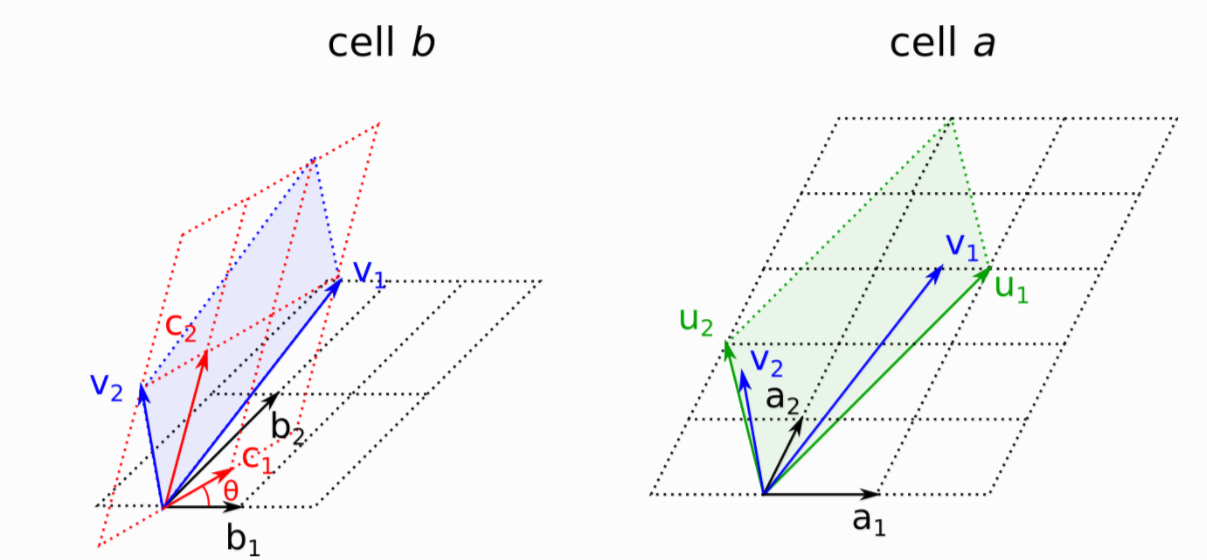
\includegraphics[width=0.6\textwidth]{cell}
\caption[Cell]{Schematic diagram for a general contact-device-contact setup\footnote{From Quantumwise.com}}
\label{fig:cell}
\end{figure}

\section*{Geometry optimization}
Relaxation of the internal coordinates of device configurations can be a tedious and time consuming task. There are two main reasons for this:
\begin{enumerate}
\item The 2-probe configuration consists of three distinct regions: Two electrodes and a central region consisting of electrode extensions and a scattering region. The geometry of each region should be separately optimized in a first-principles manner, but both electrode extensions in the central region must always match the corresponding electrode.
\item The optimum length of the central region is usually not known a priori. In the case of a periodic bulk, one would minimize the stress tensor. However, the stress field is not uniquely defined for a device configuration, so another approach is needed.
\end{enumerate}
\begin{figure}[htbp!] 
\centering    
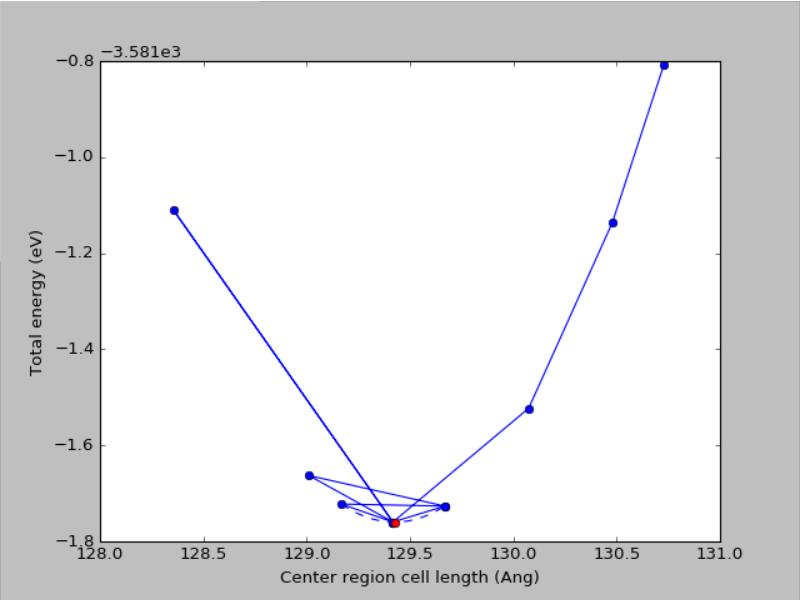
\includegraphics[width=0.6\textwidth]{optimize}
\caption[optimize]{The process of finding the central region length}
\label{fig:optimize}
\end{figure}
We must therefore rely on minimizing the device total energy while explicitly preserving the internal coordinates of the electrode extensions.Based on the $VNL$\footnote{Virtual NanoLab version 2017.0, QuantumWise A/S (www.quantumwise.com)} and $ATK$\cite{ATK1,ATK2,ATK3,ATK4} the Quantumwise provides, there are mainly two ways to do this:
\begin{enumerate}
\item \textbf{BRR}\\
After building the 2-probe configuration from fully relaxed electrodes, you extract the central region bulk and relax it with "Rigid" constraints on the atoms belonging to the electrode extensions. The device or interface is then reassembled from the relaxed bulk. This is a computationally efficient approach and will usually capture a large fraction of the required geometry relaxation. However, it does not take into account any force contributions from the electrodes, so the reassembled device may not be exactly in the global minimum-energy geometry. Some types of electronic structure calculations may be sensitive to this difference, others may not be. We shall refer to this method as Bulk Rigid Relaxation .
\item \textbf{1DMIN}\\
A somewhat more brute-force approach is to explicitly minimize the device total energy wrt. internal coordinates and the central region length, i.e., do the full 2-probe calculations and vary the central region length. This is a 1D minimization problem with relaxation of the atomic positions at each step, so we shall refer to this method as 1DMIN. We have developed a procedure for doing this as efficiently as possible with ATK, but the computations are in general more demanding than with BRR. It is therefore recommend to use 1DMIN only after pre-relaxing the central region with the BRR method. \\
We use the BRR first to conduct \textbf{Bulk Rigid Relaxation of the interface central region}, and then do \textbf{1DMIN optimization of the pre-relaxed interface using 2-probe calculations}.\\

\end{enumerate}

\noindent To search for the the central region length which corresponds minimum interface total energy,we employ a  simple \href{https://docs.scipy.org/doc/scipy-0.13.0/reference/generated/scipy.optimize.minimize_scalar.html#scipy.optimize.minimize_scalar}{SciPy} minimization procedure, whose python code is \href{https://github.com/chieko-feiyuxiao/Oric/tree/master/InterfaceOptimization}{here}.
As can be shown in Fig(\ref{fig:optimize}), the blue points are total energies of relaxed interface configurations, while the red point indicates the optimum central region length. The optimization routine simply maps out the illustrated potential-energy surface and finds its minimum.




\chapter{Tersoff Potential and Mixing rules}
\graphicspath{{Appendix3/}}
\section*{Tersoff type potentials}
As we have mentioned in the AGF method part, we need to know the position information and interaction. The former can be specified by creating and optimizing the device, but the latter must be given by some ways.\\
 Although the first principle calculations have been widely used in atomic simulations, we still choose the Tersoff type potential for the following reasons:
\begin{itemize}
\item The cost to perform first principle calculations can be quite big and even unacceptable even though several accelerating methods, for example, parallel computing can be used, which results that the first principle calculations are mainly used for very basic(which usually means 'small') systems for fundamental physics study.
\item Because we mainly focus on the III-V semi-conductors, the tersoff potential and its developments can be quite suitable for describing the interaction.(Because a large number of MD or other type of simulations have been done according to tersoff potential and many nice results have been gained)
\end{itemize}
In general, Tersoff type potentials are bond-order potentials\cite{tersoff1988new}.
They are typically used to describe covalent crystals, such as silicon, carbon, or germanium at the beginning. The potential includes two-body and three-body terms. Below we give a form of the Tersoff type potential:
\begin{equation*}
V= \sum_{i < j} f_c(r_{ij})(\chi_{R_{ij}} f_R(r_{ij})+b_{ij}f_A(r_{ij}))
\end{equation*}
which is a sum of repulsive and attractive terms
\begin{equation*}
f_R(r_{ij})=A_{ij}exp(-\lambda_{ij} r_{ij})
\end{equation*}
and
\begin{equation*}
f_A(r_{ij})=-B_{ij}exp(-\mu_{ij} r_{ij})
\end{equation*}
as well as a cutoff function
\begin{equation*}
f_C(r_{ij})=\left\{\begin{array}{ll}
1 & r_{ij}<R_{ij},\\
\frac{1}{2}+\frac{1}{2}cos(\pi \frac{r_{ij}-R_{ij}}{S_{ij}-R_{ij}}) &
R_{ij}<r_{ij}<S_{ij},\\
0 & r_{ij}>S_{ij}
\end{array}\right.
\end{equation*}
The term 
\begin{equation*}
b_{ij}=\frac{\chi_{ij}}{(1+ \beta^n \zeta_{ij}^n)^{1/2n}}
\end{equation*}
with
\begin{equation*}
\zeta_{ij}= \sum_{k \neq i,j} f_{C}(r_{ik})\omega_{ijk}exp(\alpha_{ijk}^{m_{ijk}} (r_{ij}-r_{ik})^{m_{ijk}})g(\theta_{ijk})
\end{equation*}
and
\begin{equation*}
g_{ijk}(\theta_{ijk})=1+\frac{c_{ik}^2}{d_{ik}^2}-\frac{c_{ik}^2}{[d_{ik}^2+(h- cos(\theta_{ijk}))^2]}
\end{equation*}
represents the bond order of the bond between atoms $i$ and $j$.
\section*{Mixing rule}
For more than one particle type, the following mixing rules\cite{mixing1,mixing2} are available:\\
1.$$
\lambda_{ij}=\frac{\lambda_i+\lambda_j}{2},\mu_{ij}=\frac{\mu_i+\mu_j}{2},A_{ij}=\sqrt{A_i A_j}
$$
$$
B_{ij}=\sqrt{B_i B_j},R_{ij}=\sqrt{R_i R_j}, and S_{ij}=\sqrt{S_i S_j},
$$
2.$$
\beta_{ij}=\beta_i,n_{ij}=n_i,c_{ij}=c_i,d_{ij}=d_i, and h_{ij}=h_i
$$
3.$$
\omega_{ijk}=\omega_{ij},\alpha_{ijk}=\alpha_{ij}, and m_{ijk}=m_{ij}
$$
For high-energy simulations one can modify the repulsive behavior by mixing the Tersoff potential with the universal Ziegler-Biersack-Littmark repulsive potential\cite{mixing3}
$V^{ZBL}$\\
In this case,two mixing rules are available:
\begin{itemize}
\item Type 1
$$
\bar{f}_R(r)=(1-F(r))V^{ZBL}(r)+F(r)f_R(r)
$$
\item Type 2
$$
\bar{V}_{ij}(r)=(1-F(r))V^{ZBL}(r)+F(r)V_{ij}(r)
$$
\end{itemize}
where the $F(r)$ is the Dirac-Fermi Function:
$$
F(r)=\frac{1}{1+exp(-b_f(r-r_f)}
$$







\chapter{About}
\graphicspath{{Appendix4/}}
\section*{About Me}
\textbf{Tsinghua University}\\
Undergraduate | August, 2014 - \\
\textbf{University of Tokyo}\\
Visiting student researcher|June,2017 - August, 2017\\
\begin{figure}[htbp!] 
\centering    
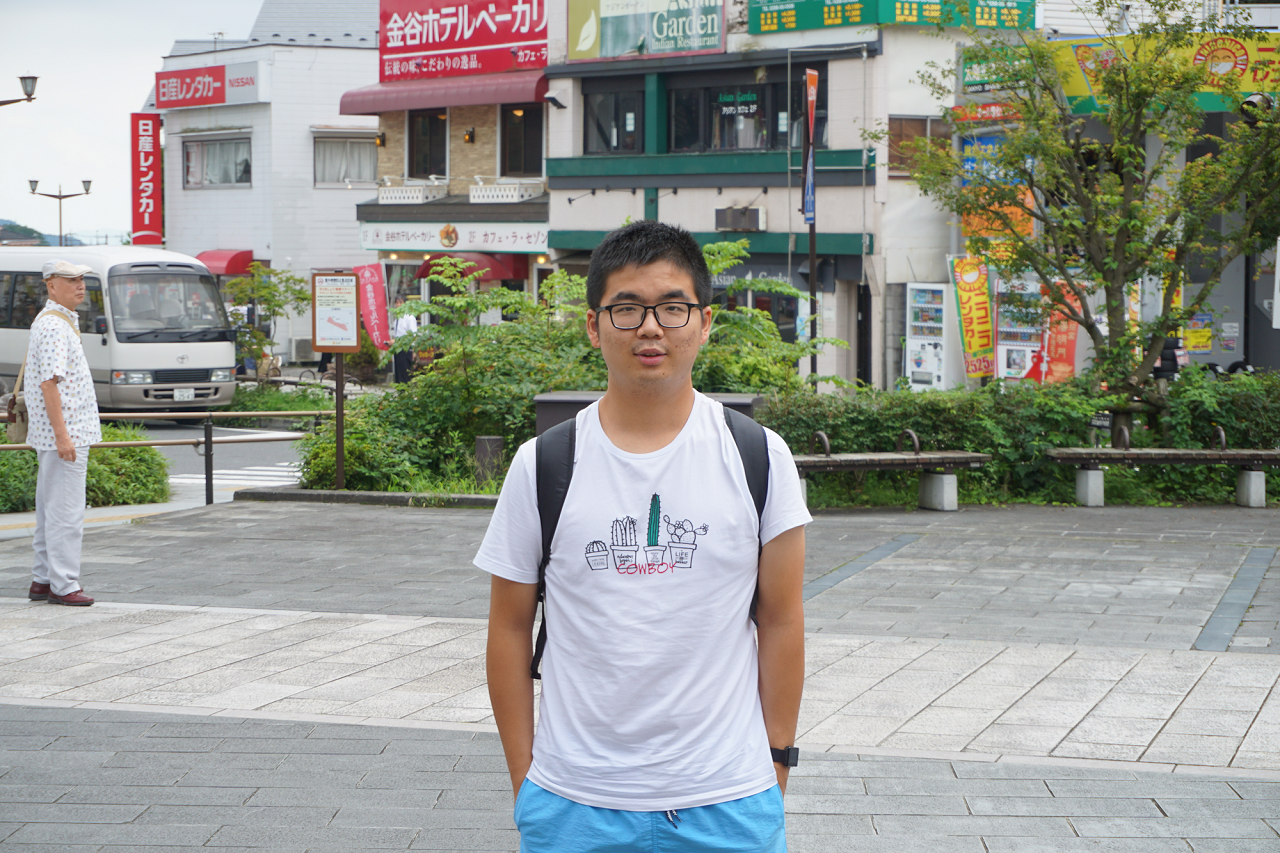
\includegraphics[width=0.8\textwidth]{xiao.png}
\caption[Xiao Feiyu]{Xiao Feiyu}
%\label{fig:cell}
\end{figure}
I show a great interest and passion in Quantum and Statistical Mechanics and have oriented my research focus on them, especially in nano materials. I've selected several related courses about it, such as Statistical Mechanics and Quantum Mechanics. During the recent months, I am doing some projects about phonon transport in nanofilms, especially their properties in interfaces. \\
\textbf{My Research}\\
I conduct my ORIC study under Prof. Bingyang Cao's guidance to learn the MC method to simulate the nano-film heat condution and do the optimization.This summer from June to Angust, I worked at Prof.Junichiro Shiomi 's Lab in Mechanical Engineering of University of Tokyo. My research topic was phonon properties at the interface using atomistic green function approach. And we also study the design and optimization of nanostructures via Bayesain optimization.\\
Tel: +86-17888830399\\
Email: xiao-14@mails.tsinghua.edu.cn\\


\section*{Supervisor: Prof. Bingyang Cao}
\begin{figure}[htbp!] 
\centering    
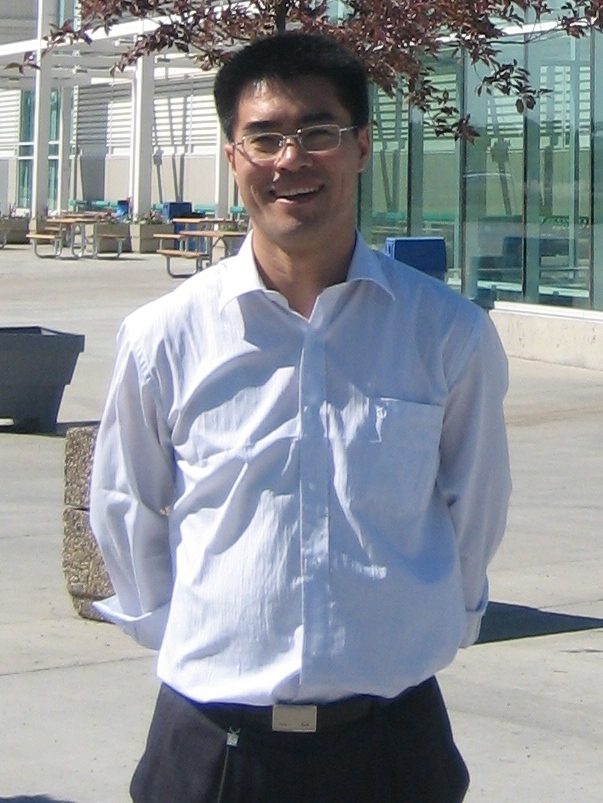
\includegraphics[width=0.3\textwidth]{Cao.png}
\caption[Prof. Bingyang Cao]{Prof. Bingyang Cao}
%\label{fig:cell}
\end{figure}
Prof. Bingyang Cao, leader of the Heatenergists Group (HEG), is also vice dean in School of Aerospace Engineering, Tsinghua University, China. His research areas are mainly focused on: (1) Non-Fourier heat transport and thermophysical properties of micro/nano-structures, including nanofilms, nanowires, nanotubes, graphene, polymer chains etc; (2) Thermal smart materials and nanocomposites with tunable or high thermal conductivity, and their applications in energy or micro/nano-electrics cooling areas; (3) Thermal management technology and theory in advanced technologies, such as nanoenergy, integrated circuits, MEMS/NEMS, laser, spacecrafts. Our work is interdisciplinary and involved in energy, aerospace, thermophysics, micro/nanofluidics and material sciences. HEG has established, as well as is seeking, extensive collaborations in research and development with universities, institutes and industries.\\
Bingyang Cao received his B.S. (1998) and M.S. (2001) from Shandong University, and Ph.D. (2005) in engineering thermophysics from Tsinghua University. He then joined Tsinghua University in 2005, and is currently a full professor and vice dean at the School of Aerospace Engineering, Tsinghua University. He also worked in Kyushu University (2005), The Hong Kong Polytechnic University (2006) and The University of Brighton (2007,2010) as a visiting professor. He has published over 100 SCI-indexed journal papers and serves as editorial board member of Scientific Reports, PLOS One, Advances in Materials Research etc. He won the New Century Excellent Talents of MOE (2011), Excellent Young Scientist Award of NSFC (2013), Zhonghua-Wu Outstanding Young Scholar Award of ETPC (2014), APL Top Reviewer Award (2017). His current research interests include non-Fourier heat conduction and thermophysical properties of nanostructures, thermal smart materials and nanocomposites, advanced thermal management technologies etc.\\
Office: Room N807, Meng Minwei S/T Building\\
Tel: +86-10-6279-4531\\
Email: caoby@tsinghua.edu.cn\\
\section*{Prof. Junichiro Shiomi}
\begin{figure}[htbp!] 
\centering    
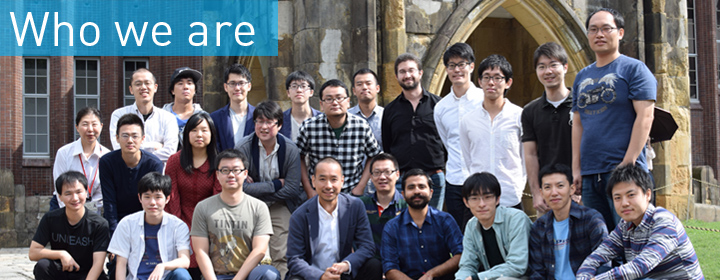
\includegraphics[width=0.8\textwidth]{shiomi.png}
\caption[Prof. Junichiro Shiomi]{Prof. Junichiro Shiomi's lab}
%\label{fig:cell}
\end{figure}
 Prof. Junichiro Shiomi received the B.E. (1999) from Tohoku University, and Ph. D. (2004) from Royal Institute of Technology (KTH), Sweden. He is currently a Professor in Department of Mechanical Engineering, The University of Tokyo. His research interests include heat conduction of nanomaterials, polymer composites, and thermoelectrics, phase change and fluidics in nanoscale, interfacial thermofluid dynamics, thermal convections, and materials informatics. He is a recipient of the Zeldovich Medal from the Committee on Space Research, Young Scientists' Prize, the Commendation for Science and Technology by the Minister of Educational, Culture, Sports, Science and Technology, and the Academic award of Heat Transfer Society of Japan. \\ 
Email: shiomi@photon.t.u-tokyo.ac.jp


\end{appendices}

% *************************************** Index ********************************
\printthesisindex % If index is present

\end{document}

